\documentclass{article}
\usepackage[english,activeacute]{babel}
\usepackage{listings}
\usepackage[utf8]{inputenc}
\usepackage{amsmath,amsfonts,amssymb,amstext,amsthm,amscd}
\usepackage{graphicx}
\usepackage{float}
\usepackage{here} %usar el comandao[H] Para fijar la posición de las imágenes
\usepackage{multicol}
\graphicspath{{Imagenes/}}
% Estilo de página y encabezados 
% --------------------------------------------------------------------------------------------------------------------------------------------------------------
\usepackage{fancyhdr}
\setlength{\headheight}{15.2pt}
\usepackage[paperwidth=8.5in, paperheight=11.0in, top=1.0in, bottom=1.0in, left=1.0in, right=1.0in]{geometry}  
\pagestyle{fancyplain}
\fancyhead[R]{LRT2022 Digital design}
\fancyhead[C]{}
\fancyhead[L]{Fall 2025}
\fancyfoot[L]{}
\fancyfoot[C]{\thepage}
\fancyfoot[R]{}
% --------------------------------------------------------------------------------------------------------------------------------------------------------------
% Inicio del documento
\begin{document}
\fancypagestyle{plain}{
    \renewcommand{\headrulewidth}{1pt}
    \renewcommand{\footrulewidth}{1pt}
}
\renewcommand{\footrulewidth}{1pt}
\renewcommand{\tablename}{Tabla}
% --------------------------------------------------------------------------------------------------------------------------------------------------------------
%Titulo y autor
\author{}% 
\title{Report 5: Combinational Logic Circuits (Individual Assignment)}% 
\date{Sección 7}% 
\maketitle
% --------------------------------------------------------------------------------------------------------------------------------------------------------------
% Escribir resumen 150-200 palabras
\begin{abstract}
This report presents the results obtained in the fifth laboratory practice of the Digital Design course. The main objective of this practice was to initiate the development of projects on FPGA, continuing with the use of the VHDL language as a programming tool. The practice focused on the implementation and simulation of combinational logic circuits using both schematic diagrams and Boolean functions. Likewise, three exercises were designed: tank control, coin detection, and the Rock, Paper, Scissors game, all developed in VHDL with the purpose of applying the concepts of logic design and strengthening programming and digital simulation skills. 
\end{abstract}

% --------------------------------------------------------------------------------------------------------------------------------------------------------------
\begin{multicols}{2} %Documento a dos columnas
\section{Introduction}\label{Intro}  
Combinational logic circuits are digital systems whose output depends exclusively on the combinations present at the inputs, without using storage elements or feedback. Unlike sequential circuits, in which the outputs depend on the history of previous states, combinational circuits produce instant results based on the applied logical conditions. This principle makes them essential components within digital electronics, as they allow the implementation of arithmetic operations, encoders, decoders, multiplexers, and other fundamental blocks of modern digital systems. 

The design of combinational circuits is based on Boolean algebra, a branch of mathematics that uses binary variables and logical operations to describe the behavior of digital systems. Through the simplification of Boolean expressions and the implementation of minimal logic functions, it is possible to optimize circuits in terms of speed, cost, and resource consumption. Tools such as Karnaugh maps and algebraic methods are widely used to reduce logic functions to their most efficient forms. 

Currently, the VHDL language (VHSIC Hardware Description Language) has consolidated as a standard tool for the description, simulation, and synthesis of digital circuits. VHDL allows structural or behavioral representation of electronic system operation, facilitating verification before physical implementation. Moreover, its compatibility with reconfigurable hardware platforms, such as FPGAs (Field Programmable Gate Arrays), makes it an essential tool in the development of high-complexity digital projects.During this laboratory practice, the fundamentals of combinational logic design were applied through the creation of three projects: 
A water tank control system, which automates the filling of a tank using level sensors. 
A coin detector, capable of identifying different denominations based on signals generated by photodiodes. 
A digital Rock, Paper, Scissors game, designed with combinational logic to determine the outcome of each match according to the players’ moves. 

These exercises allowed the integration of theoretical concepts of Boolean algebra, logic design, and digital modeling in VHDL, strengthening the analysis, synthesis, and simulation skills necessary for the development of digital systems on FPGA. 

\section{Objectives}\label{Objectives}  
The objectives of this practice are: 
\begin{itemize}
  \item To design combinational logic circuits representing different digital applications. 
  \item To program and simulate the designed circuits using the VHDL language to verify their functionality. 
\end{itemize}
To achieve these objectives, it is essential to understand the structure and operation of combinational circuits, which process binary input signals to generate defined logical results without depending on time or previous state. Their design starts from the analysis of Boolean functions that describe the relationship between inputs and outputs, which can be simplified to optimize implementation. Likewise, the use of VHDL as a hardware description tool allows simulating circuit behavior before physical construction, ensuring a functional and efficient design. 

\section{Methodology}\label{Meth}
The methodology applied in this laboratory practice was structured into three main phases: logical analysis, simulation in EDA Playground, and physical implementation on the Basys 3 board.This procedure was carried out systematically for each of the required exercises, ensuring the correct application of digital design from the theoretical stage to practical verification. 

\subsection{Logical Analysis Phase}
During this first stage, the following activities were carried out:
\begin{enumerate}
    \item The truth tables or functional requirements corresponding to each of the proposed circuits were analyzed. Based on this information, the necessary input-output relationships were identified to meet the expected behavior and obtain a solution for each problem. 
    \item The results obtained were carefully documented for use in the subsequent simulation and programming phases. 
\end{enumerate}

\subsection{EDA Playground Simulation Phase}
In the EDA Playground digital simulation environment, the following procedures were performed: 
\begin{enumerate}
    \item The combinational circuits were programmed in VHDL, ensuring that the description of logical behavior matched the defined functional requirements. 
    \item Verification testbenches were developed to check the operation of each design and validate the system responses to different input combinations. 
    \item Simulation results were compared with the original truth tables, ensuring correct logical implementation. 
    \item The obtained waveforms were recorded, showing consistency between the theoretical design and the digital simulation. 
\end{enumerate}

\subsection{Basys 3 Board Implementation Phase}
Finally, the physical implementation of the circuits was carried out on the Basys 3 board, following the steps described below: 
\begin{enumerate}
    \item The VHDL code of each circuit was synthesized, and the necessary bitstream (.bit) files were generated for programming in Vivado. 
    \item Pin constraints (.xdc) were assigned, mapping the logical signals to the physical components of the board (switches, LEDs, and displays). 
    \item The designs were loaded onto the Basys 3, verifying their correct operation through practical input-output tests. 
    \item The correspondence between the physically obtained results and the previous simulations was verified, confirming the correct behavior of the combinational circuits designed in each exercise. 
\end{enumerate}

\section{Results}\label{Results}

\subsection{Rock Paper Scissors Game}\label{R,P,S Game}
For the Rock, Paper, Scissors game circuit, a combinational system was designed with five inputs (PB, JAA, JAB, JBA, JBB) and a three-bit output vector (salida). The inputs correspond to buttons or switches that allow the players to choose their move: 
PB: game start button. 
JAA and JAB: Player A’s selection. 
JBA and JBB: Player B’s selection. 
The output salida indicates the game result encoded in three bits, where each combination represents a specific condition, such as a player victory, a tie, or the game not started. For this circuit, the following truth table was developed, showing the relationship between the inputs and the output: 

\begin{table}[H]
\centering
\begin{tabular}{|c|c|c|c|c|}
\hline
\multicolumn{5}{|c|}{\textbf{Input}} \\
\hline
\textbf{PB} & \textbf{JAA} & \textbf{JAB} & \textbf{JBA} & \textbf{JBB} \\
\hline
1 & 0 & 0 & 0 & 0 \\
1 & 0 & 0 & 0 & 1 \\
1 & 0 & 0 & 1 & 0 \\
1 & 0 & 0 & 1 & 1 \\
1 & 0 & 1 & 0 & 0 \\
1 & 0 & 1 & 0 & 1 \\
1 & 0 & 1 & 1 & 0 \\
1 & 0 & 1 & 1 & 1 \\
1 & 1 & 0 & 0 & 0 \\
1 & 1 & 0 & 0 & 1 \\
1 & 1 & 0 & 1 & 0 \\
1 & 1 & 0 & 1 & 1 \\
1 & 1 & 1 & 0 & 0 \\
1 & 1 & 1 & 0 & 1 \\
1 & 1 & 1 & 1 & 0 \\
1 & 1 & 1 & 1 & 1 \\
\hline
\end{tabular}
\caption{Input Combinations for ent\_juego (Adapted from )}
\label{tab:vhdl_juego_inputs}
\end{table}

\begin{table}[H]
\centering
\begin{tabular}{|c|c|c|}
\hline
\multicolumn{3}{|c|}{\textbf{Output (SAL)}} \\
\hline
\textbf{E} & \textbf{GJA} & \textbf{GJB} \\
\hline
0 & 0 & 0 \\
0 & 0 & 0 \\
0 & 0 & 0 \\
0 & 0 & 0 \\
0 & 0 & 0 \\
1 & 0 & 0 \\
0 & 0 & 1 \\
0 & 1 & 0 \\
0 & 0 & 0 \\
0 & 1 & 0 \\
1 & 0 & 0 \\
0 & 0 & 1 \\
0 & 0 & 0 \\
1 & 0 & 0 \\
0 & 1 & 0 \\
1 & 0 & 0 \\
\hline
\end{tabular}
\caption{Corresponding Outputs for ent\_juego (Adapted from )}
\label{tab:vhdl_juego_outputs}
\end{table}
And based on these truth tables, a code was generated in VHDL to simulate and implement the circuit. The code is shown below:
\lstinputlisting[language=VHDL, caption=VHDL Code for Water Pump Program, label=lst:vhdl_juego]{codigos/VHDL/Cisterna/design.vhd}
From which, the following testbench was created to verify the functionality of the code:
\lstinputlisting[language=VHDL, caption=VHDL Testbench for Water Pump Program, label=lst:vhdl_tb_juego]{codigos/VHDL/Cisterna/testbench.vhd}
After verifying the table, the corresponding VHDL code was reviewed, simulations were carried out in EpWave, and finally it was implemented on the Basys 3, where the game results could be observed through LEDs. 

\begin{figure}[H]
  \centering
  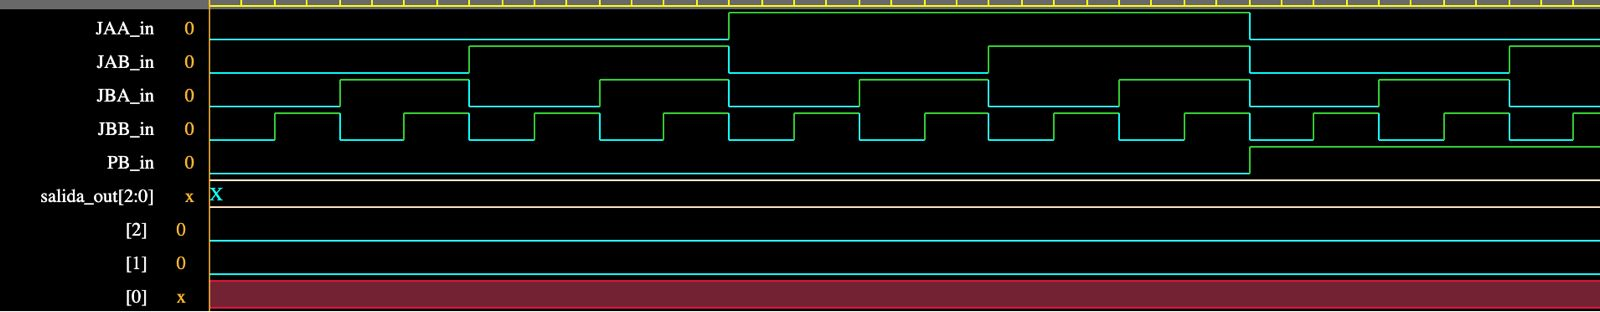
\includegraphics[width = 0.5\textwidth]{ppt.jpg}
  \caption{EDA Waves Simulation for Rock, Paper, Scissors Game}
  \label{fig:lab_cis_eda}
\end{figure}
\begin{figure}[H]
  \centering
  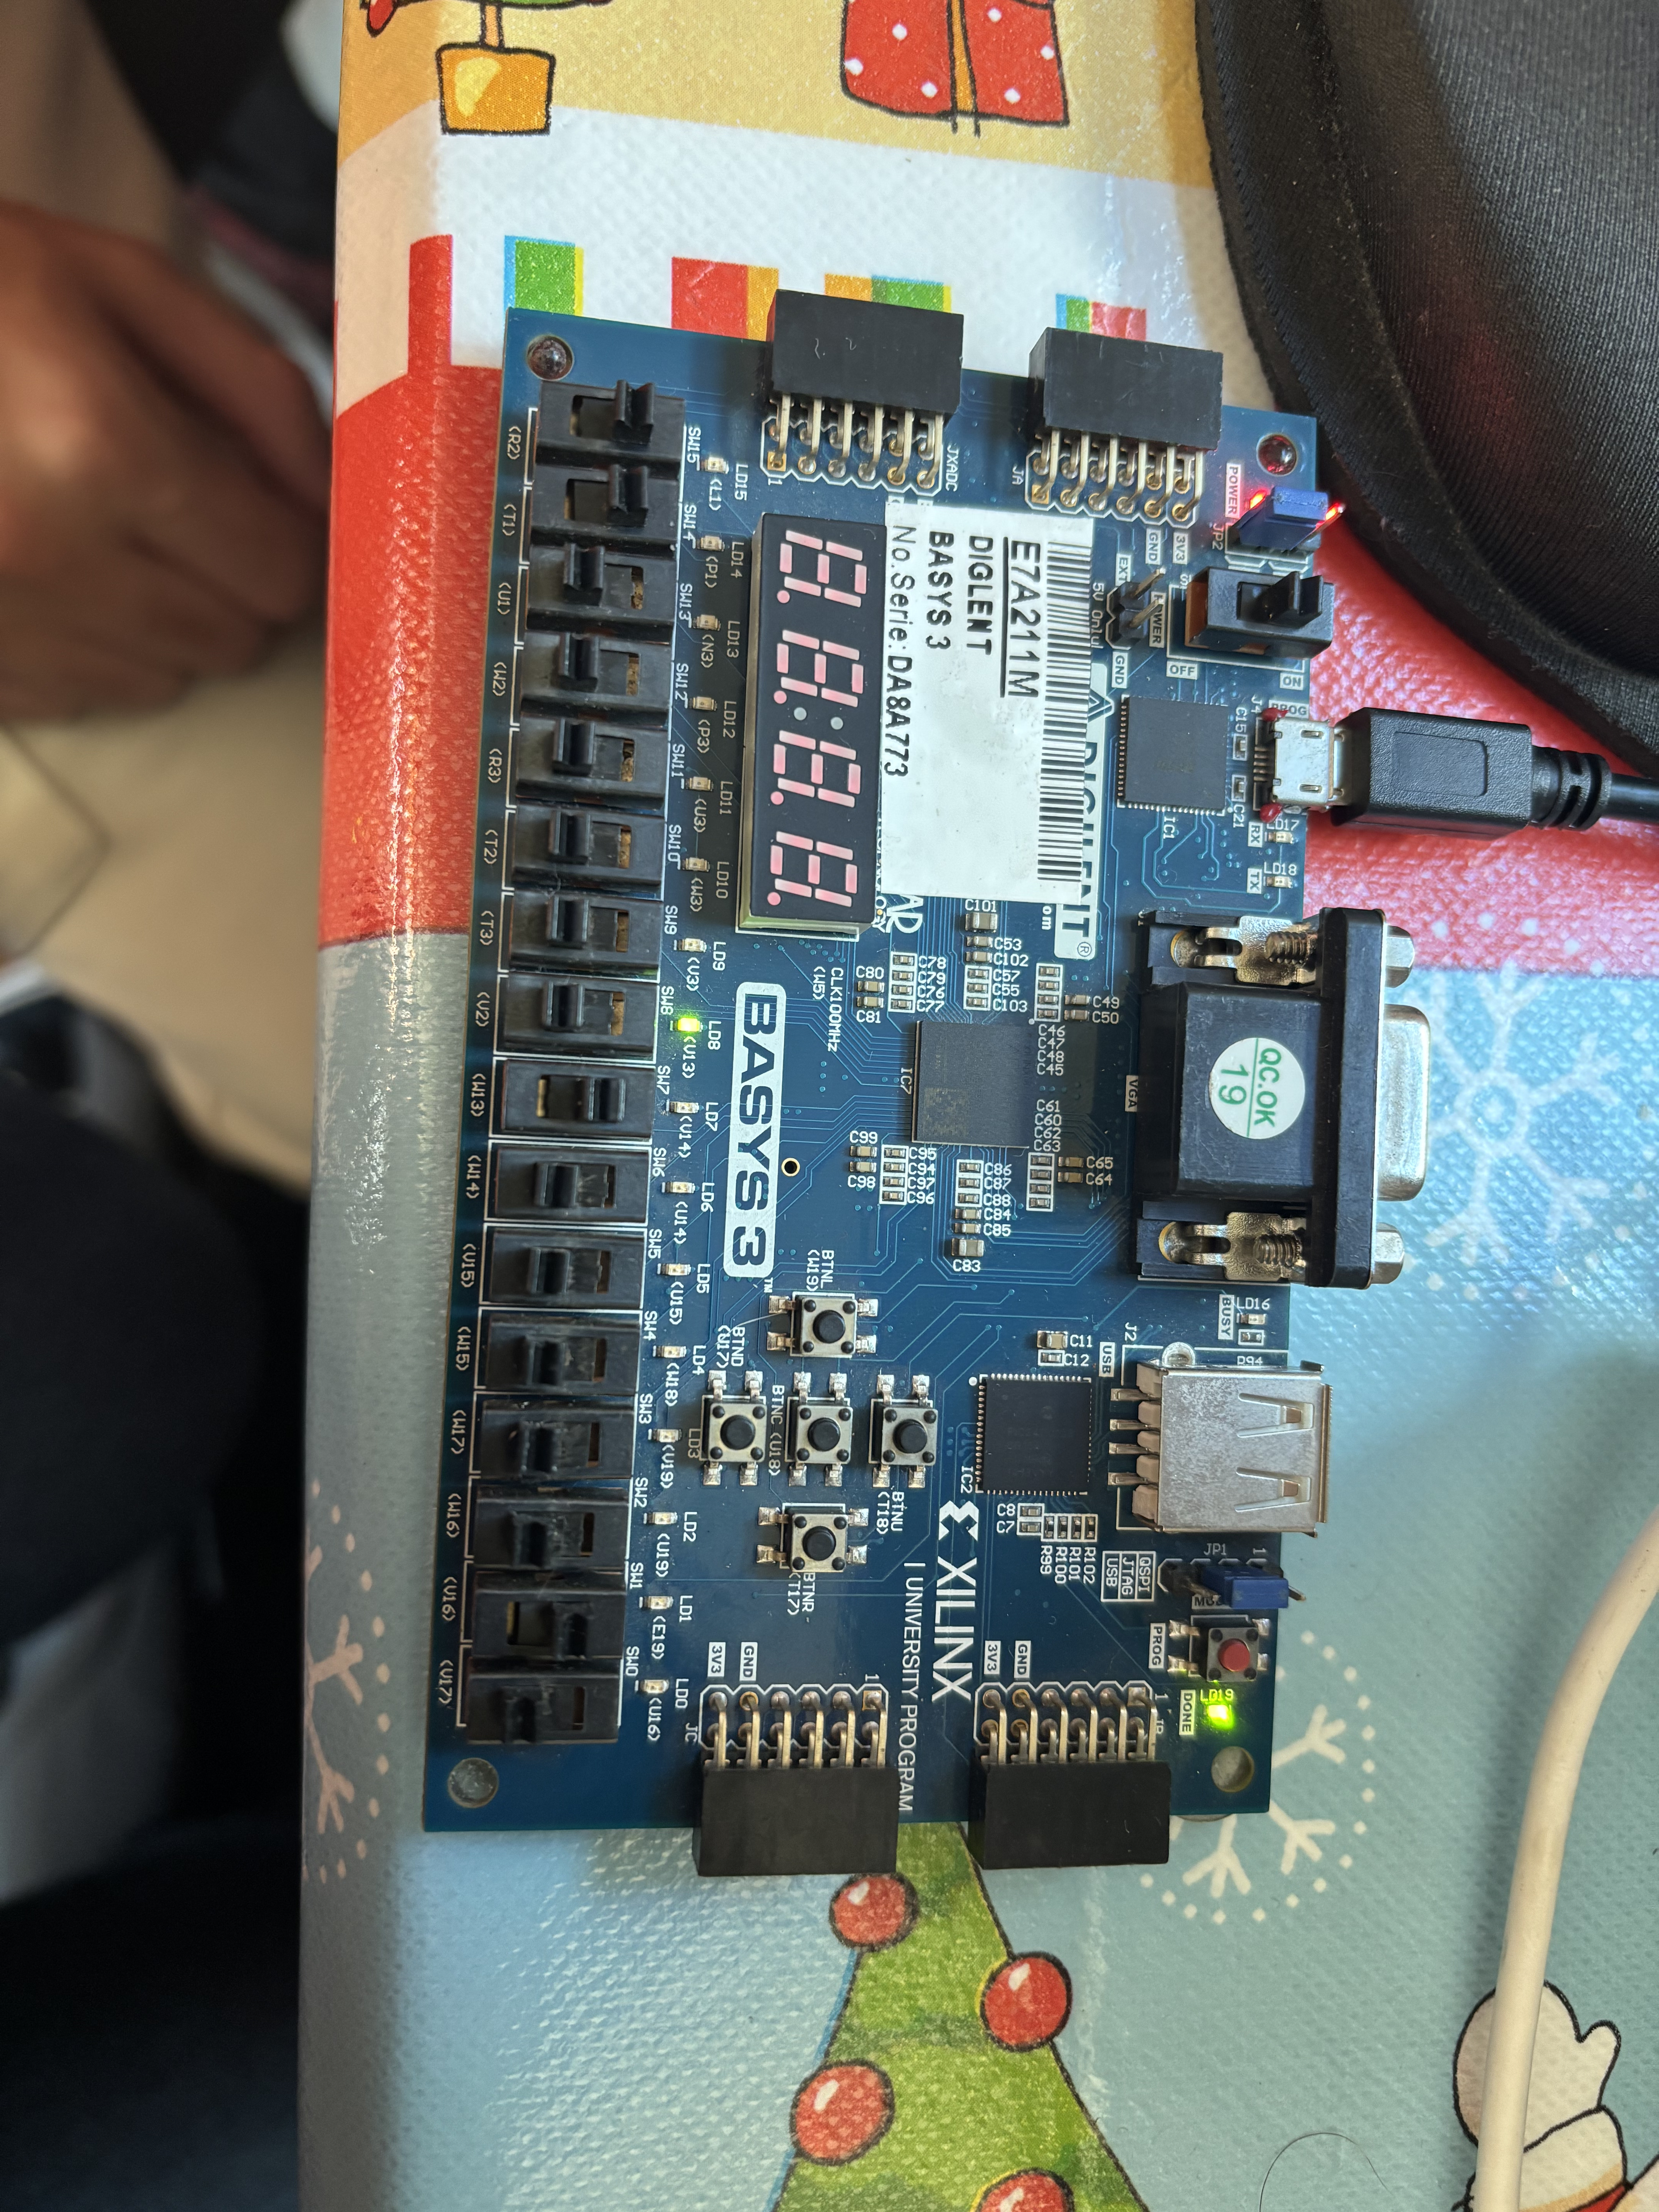
\includegraphics[width = 0.3\textwidth]{AWIN.jpg}
  \caption{Basys 3 Board Implementation of the Rock, Paper, Scissors Game when A wins }
  \label{fig:AWIN}
\end{figure}
\begin{figure}[H]
  \centering
  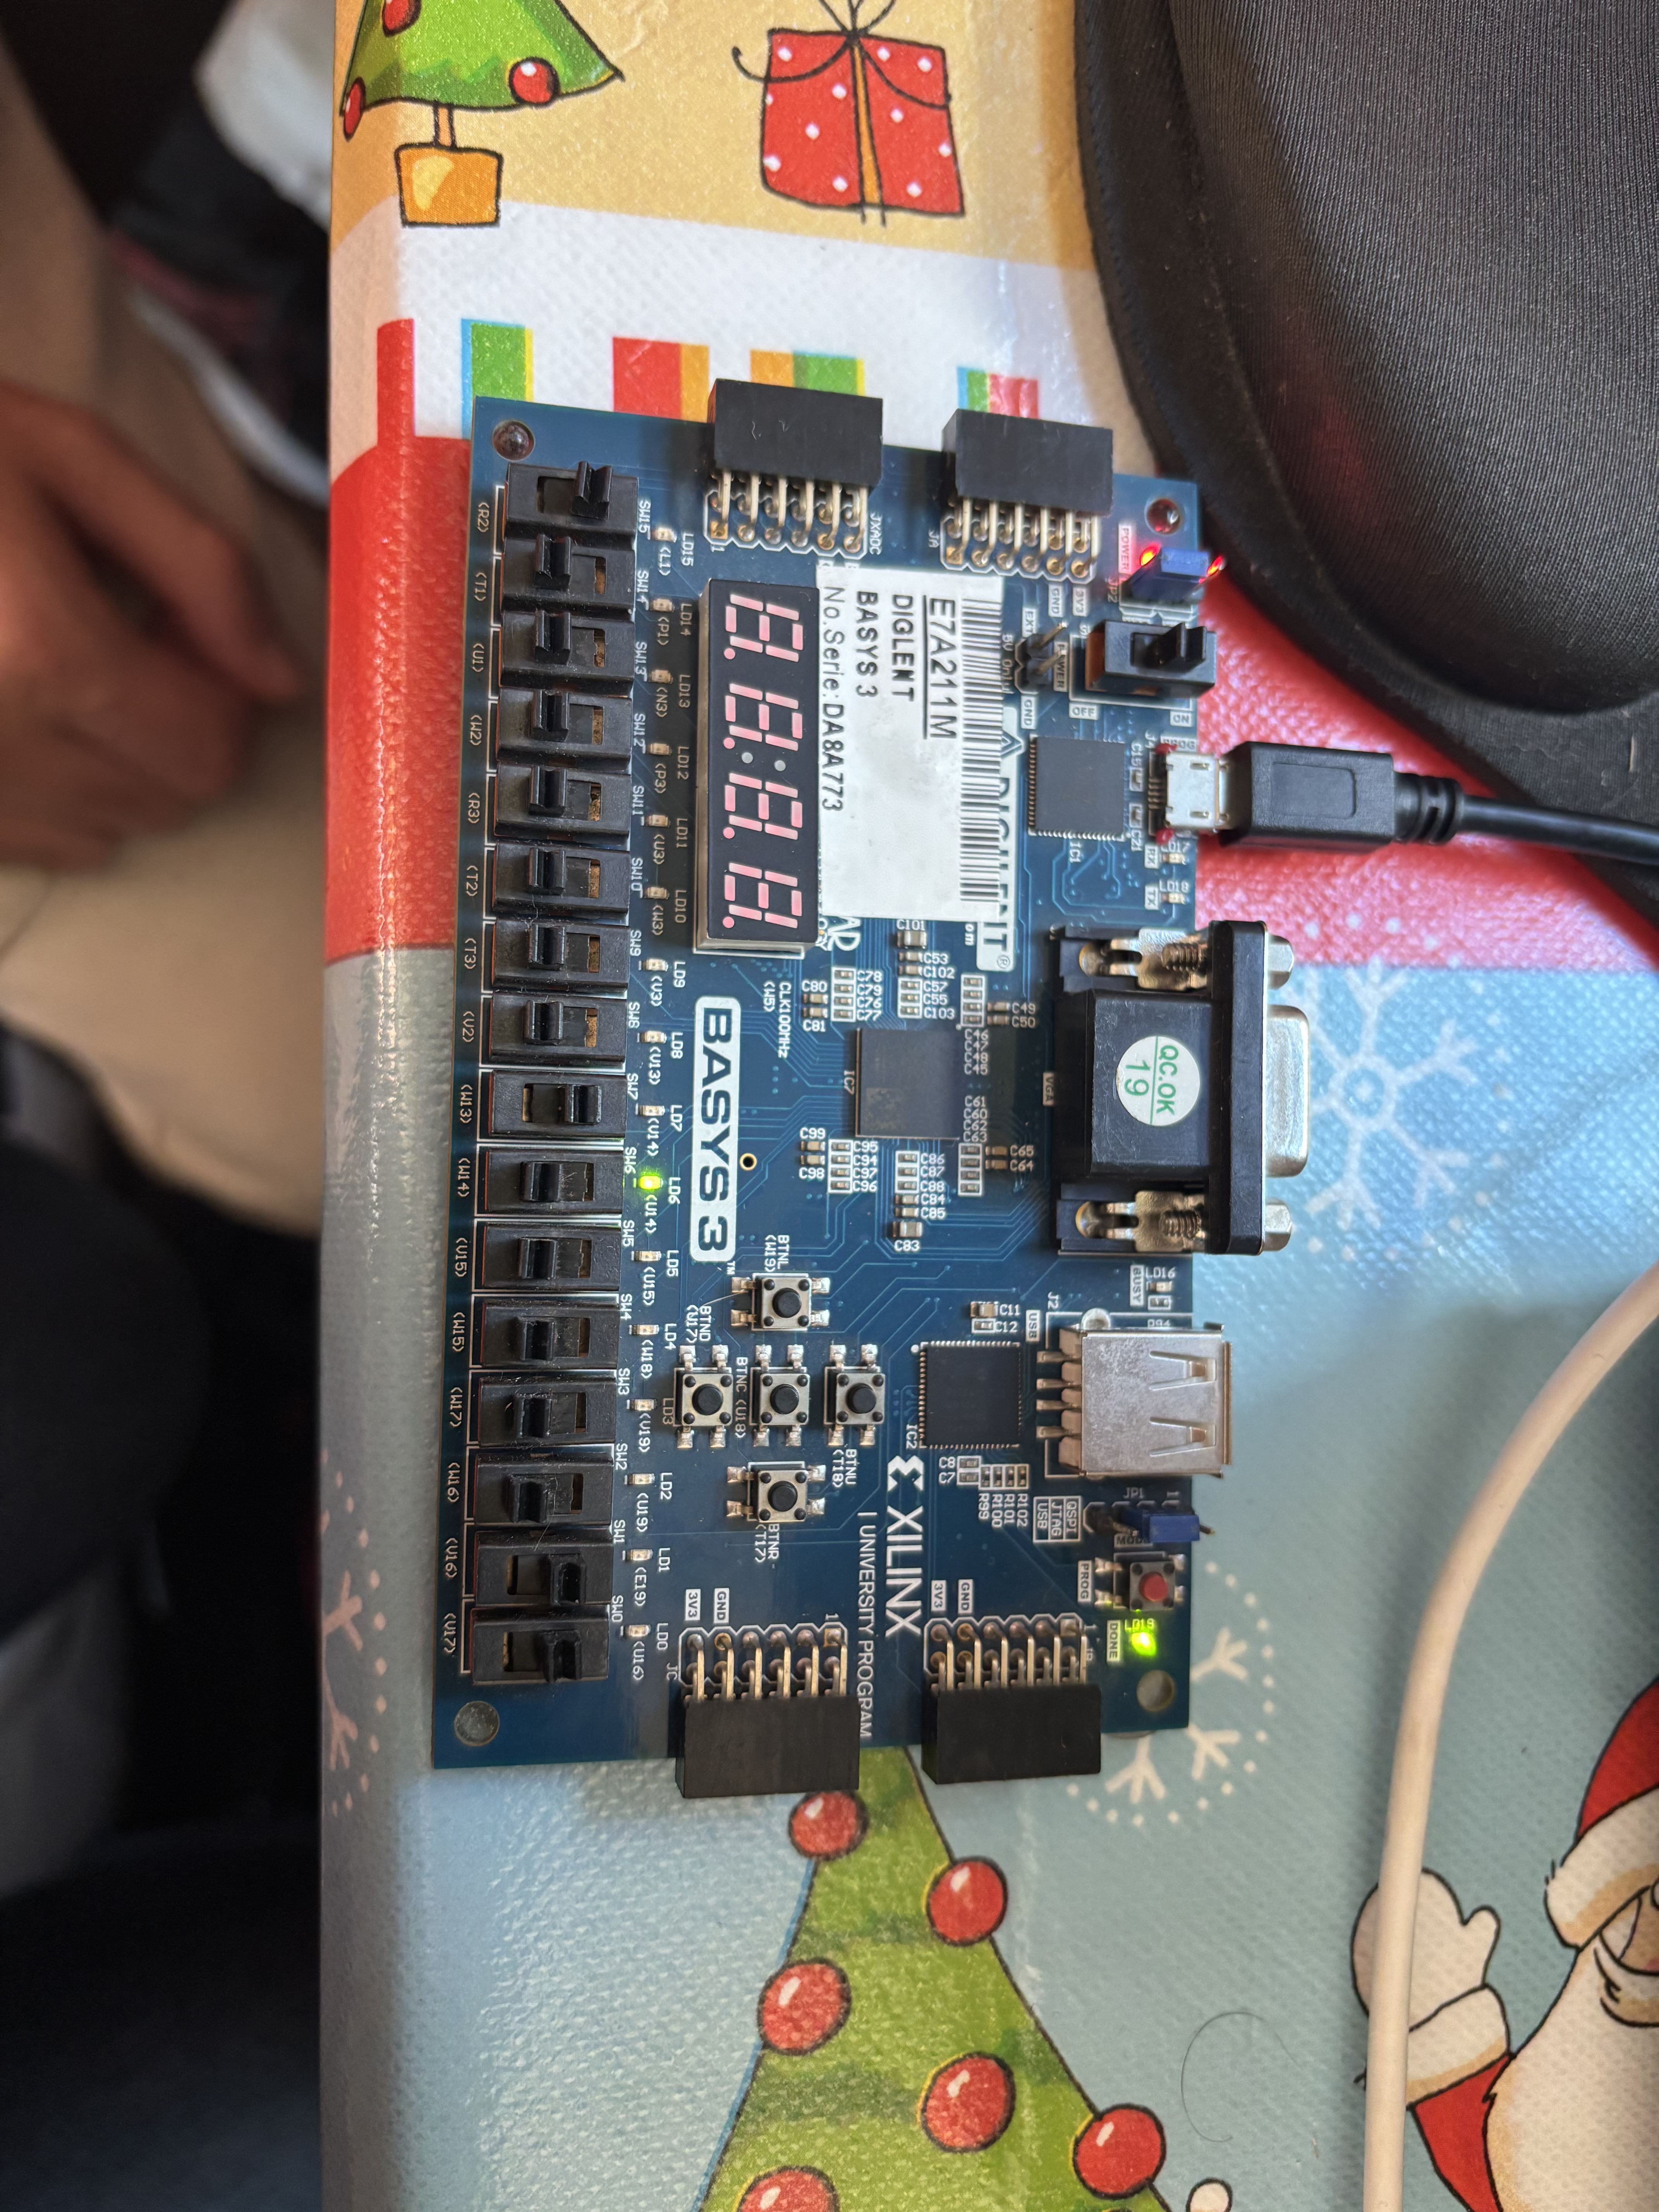
\includegraphics[width = 0.3\textwidth]{BWIN.jpg}
  \caption{Basys 3 Board Implementation of the Rock, Paper, Scissors Game when B wins }
  \label{fig:bwin}
\end{figure}
\begin{figure}[H]
  \centering
  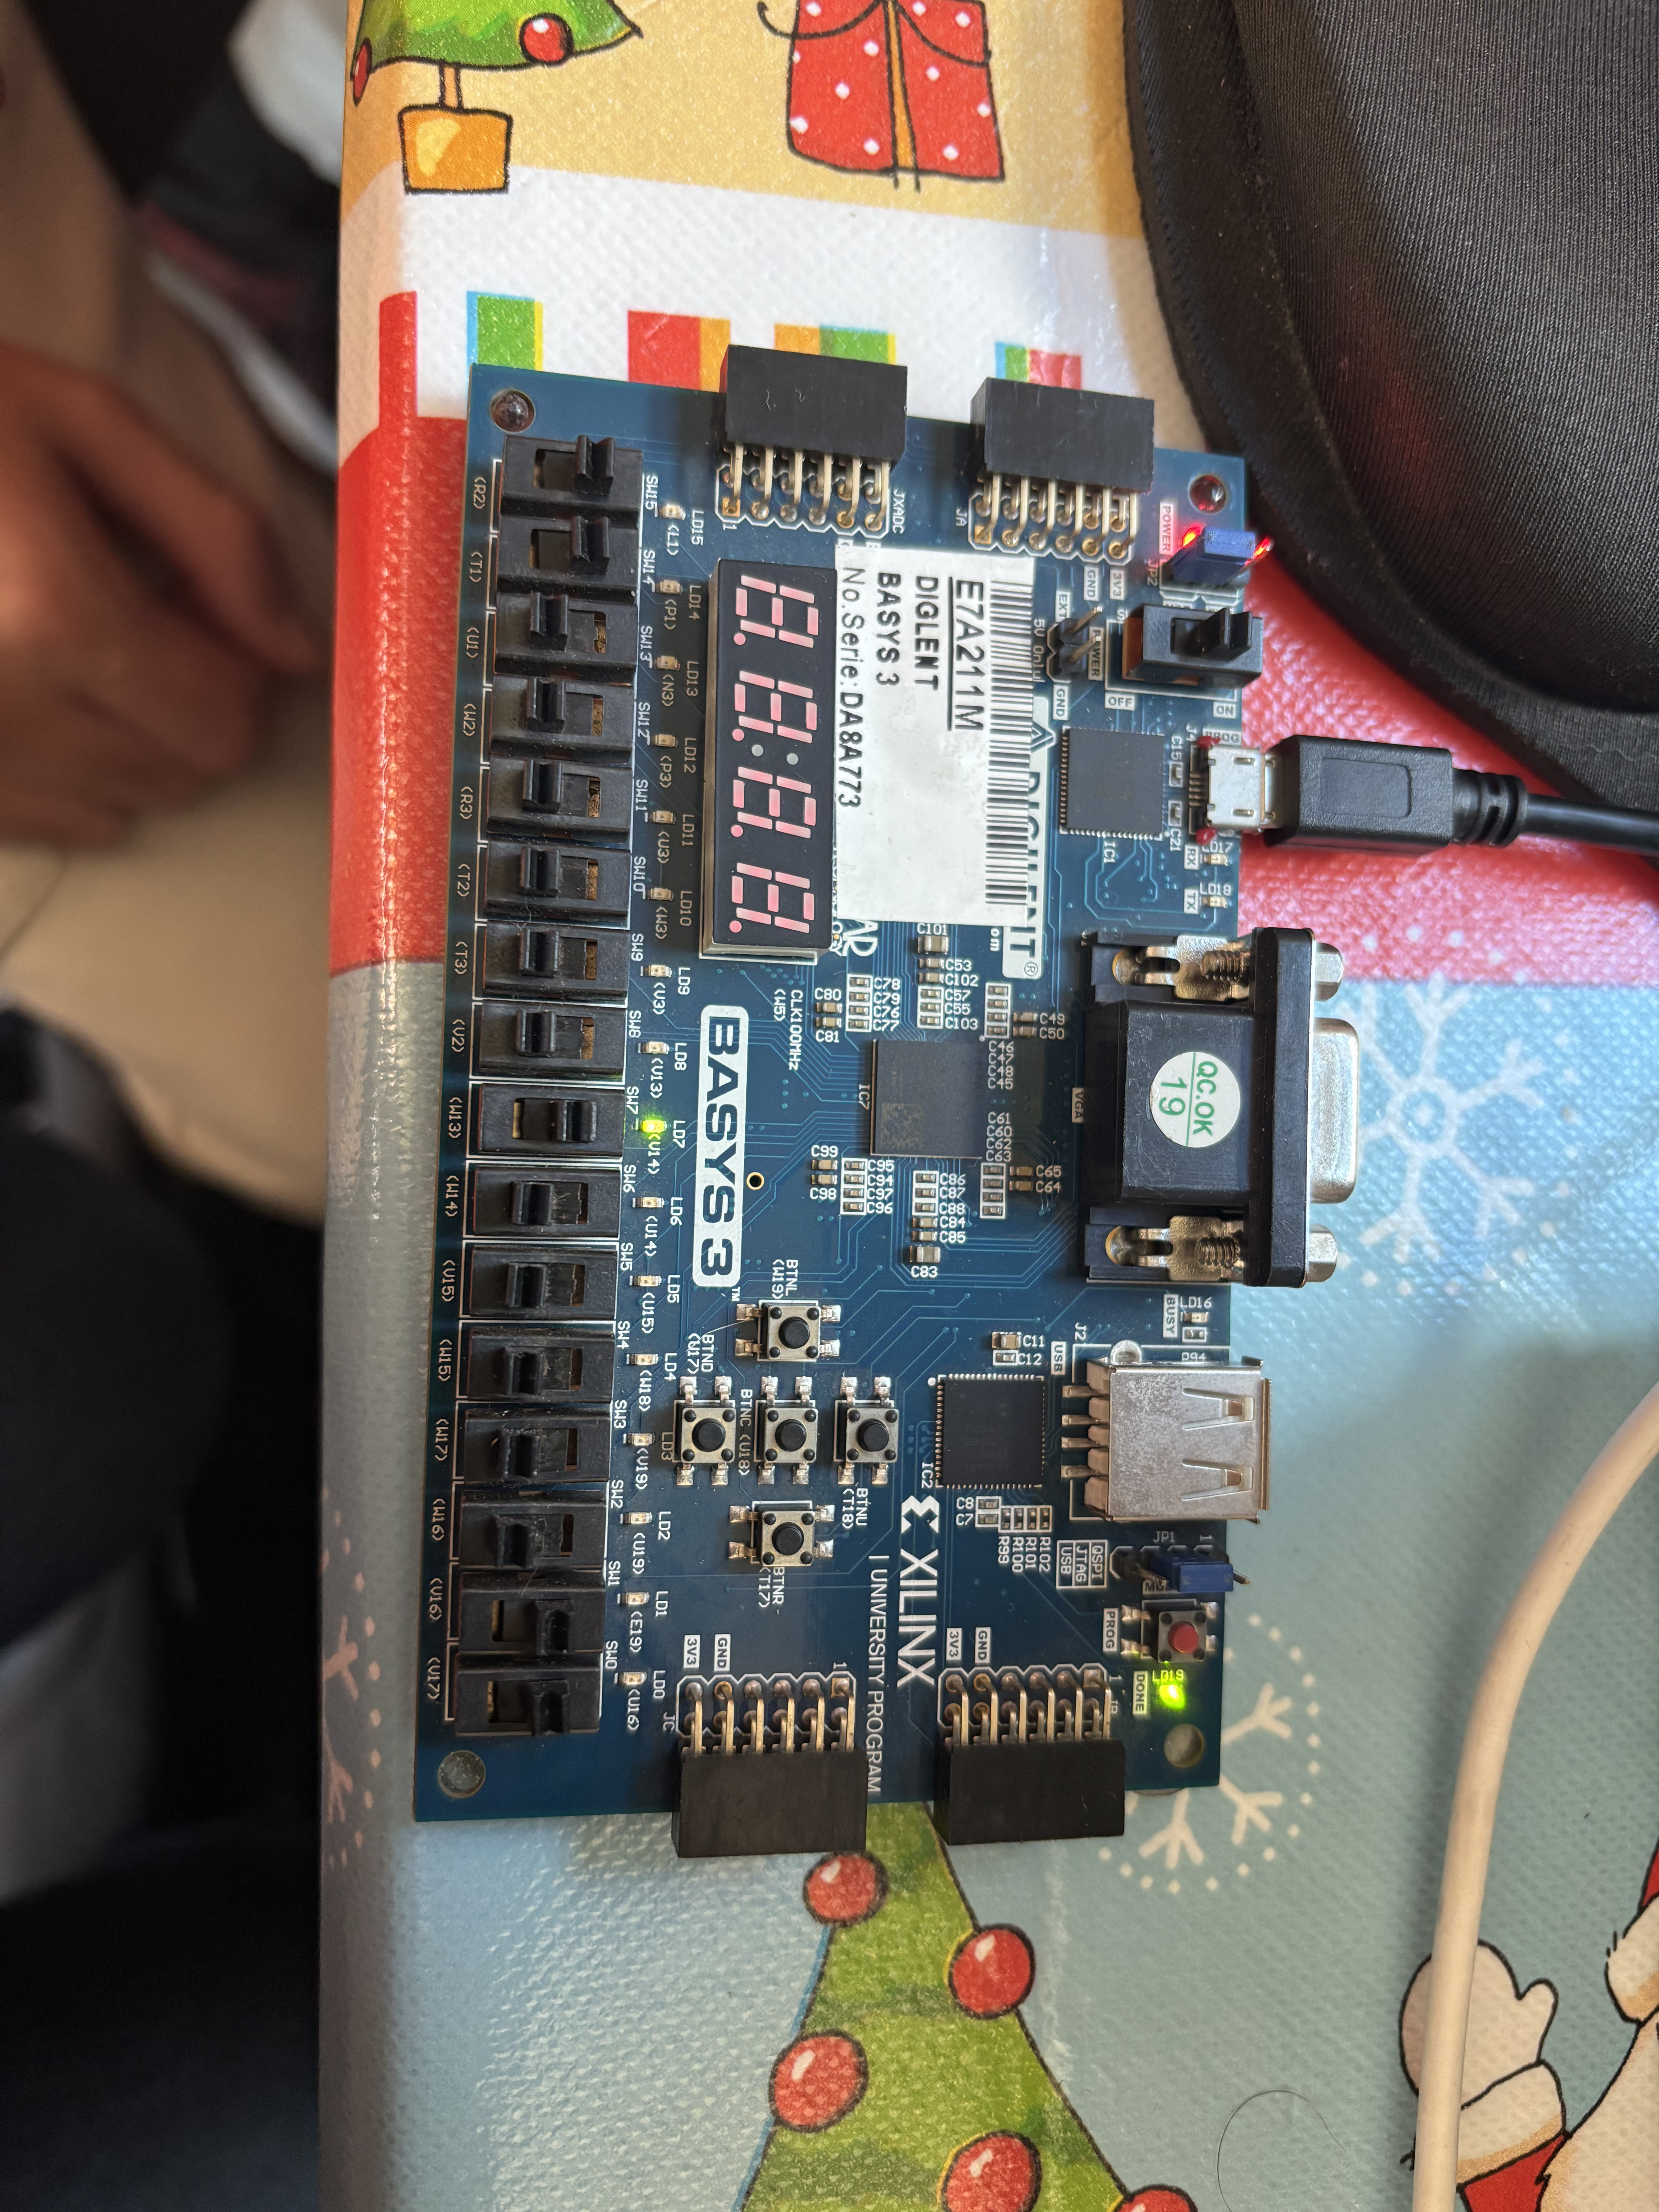
\includegraphics[width = 0.3\textwidth]{TIE.jpg}
  \caption{Basys 3 Board Implementation of the Rock, Paper, Scissors Game in Case of a Tie }
  \label{fig:tie}
\end{figure}

\subsection{Water Pump}\label{Cisterna}
For the cistern and tank filling control system, a combinational system was designed with four inputs (A, B, C, D) and one output (M). Inputs A and B correspond to the high and low level sensors of the tank, respectively. Inputs C and D correspond to the high and low level sensors of the cistern. The output M controls the pump motor, activating only when the cistern has water and the tank is not full. The following truth table shows the system behavior for all possible input combinations: 

\begin{table}[H]
\centering
\begin{tabular}{|c|c|c|c|c|}
\hline
\textbf{A} & \textbf{B} & \textbf{C} & \textbf{D} & \textbf{M} \\ \hline
0 & 0 & 0 & 0 & 0 \\
0 & 0 & 0 & 1 & 1 \\
0 & 0 & 1 & 0 & 0 \\
0 & 0 & 1 & 1 & 1 \\
0 & 1 & 0 & 0 & 0 \\
0 & 1 & 0 & 1 & 1 \\
0 & 1 & 1 & 0 & 0 \\
0 & 1 & 1 & 1 & 1 \\
1 & 0 & 0 & 0 & 0 \\
1 & 0 & 0 & 1 & 0 \\
1 & 0 & 1 & 0 & 0 \\
1 & 0 & 1 & 1 & 0 \\
1 & 1 & 0 & 0 & 0 \\
1 & 1 & 0 & 1 & 0 \\
1 & 1 & 1 & 0 & 0 \\
1 & 1 & 1 & 1 & 0 \\ \hline
\end{tabular}
\caption{Combinations for Water Pump Controller }
\label{tab:water_pump}
\end{table}

The simplified boolean expression obtained was: 
\begin{equation}
  \mathbf{M} = \neg A \cdot D
\end{equation}
And based on these truth tables, a code was generated in VHDL to simulate and implement the circuit. The code is shown below:
\lstinputlisting[language=VHDL, caption=VHDL Code for Water Pump Program, label=lst:vhdl_juego]{codigos/VHDL/Cisterna/design.vhd}
From which, the following testbench was created to verify the functionality of the code:
\lstinputlisting[language=VHDL, caption=VHDL Testbench for Water Pump Program, label=lst:vhdl_tb_juego]{codigos/VHDL/Cisterna/testbench.vhd}
Finally, the VHDL code was verified, simulated in EpWave, and implemented on the Basys 3, where the activation of the motor could be physically observed through LEDs or other indicators. 

\begin{figure}[H]
  \centering
  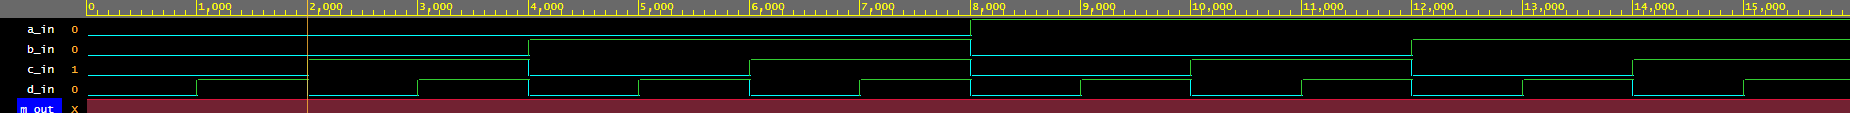
\includegraphics[width = 0.5\textwidth]{Cis.png}
  \caption{EDA Waves Simulation for Water Pump Controller }
  \label{fig:lab_cis_eda}
\end{figure}
\begin{figure}[H]
  \centering
  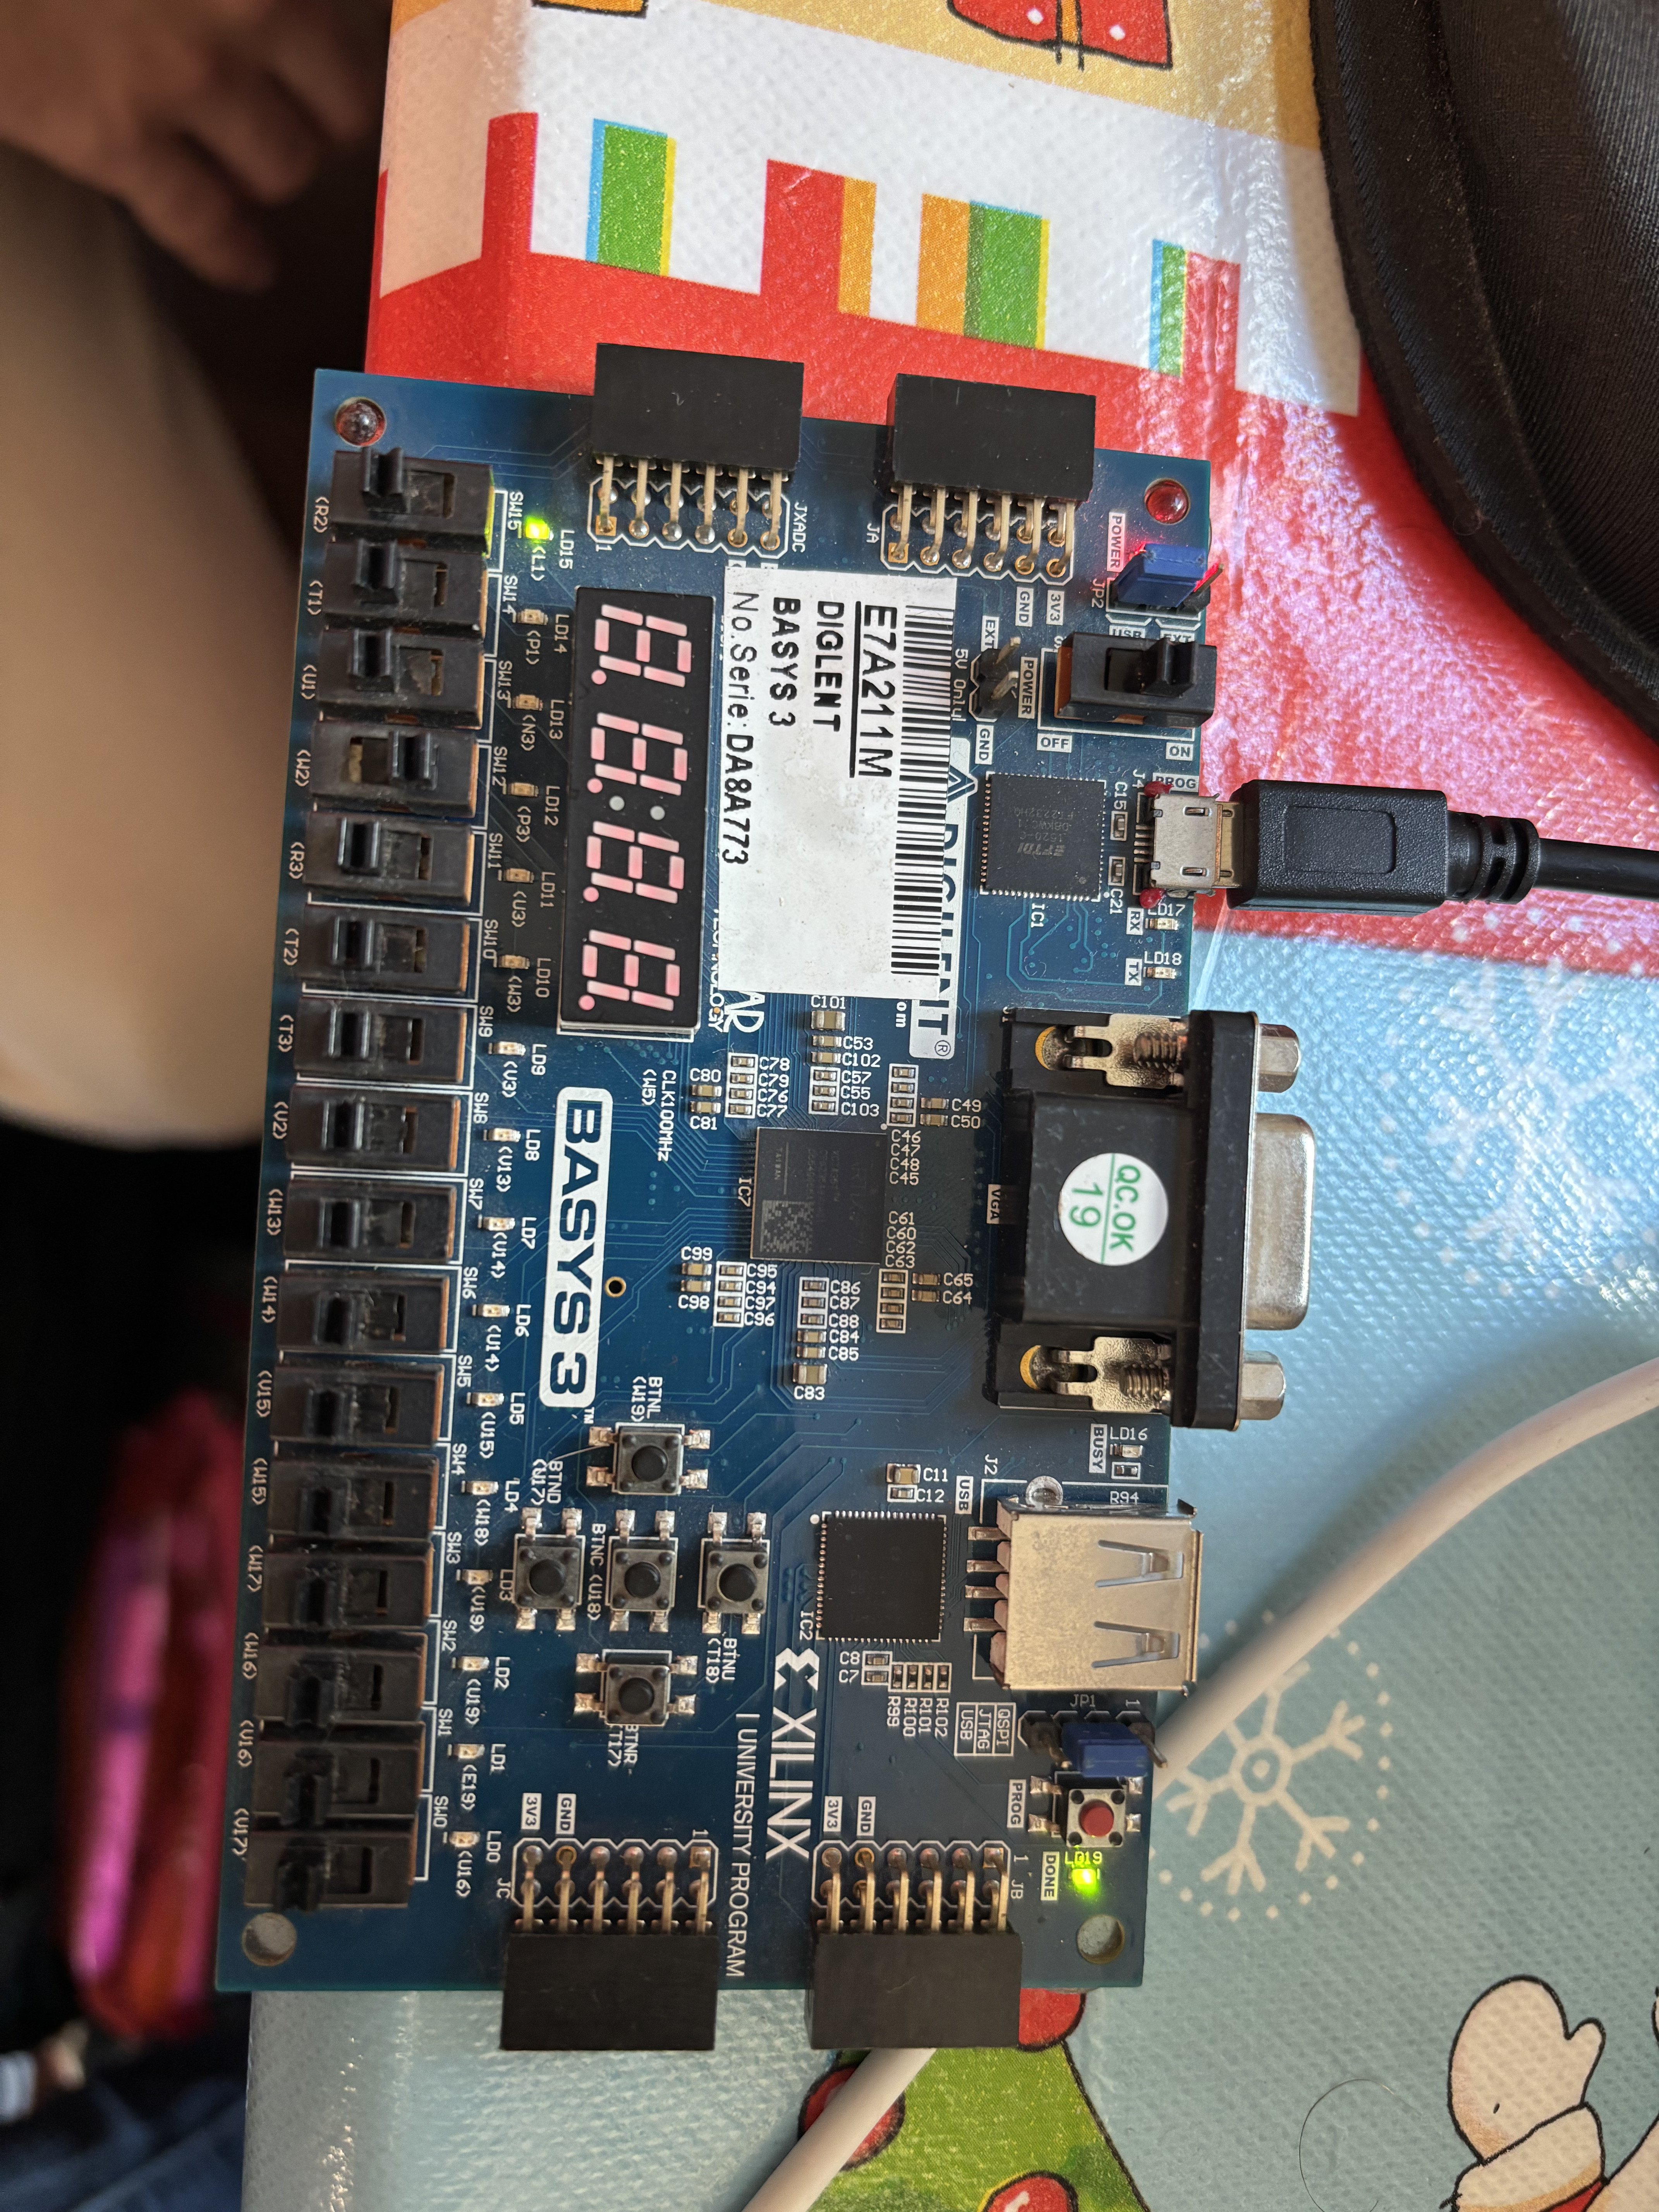
\includegraphics[width = 0.3\textwidth]{ONCIS1.jpg}
  \caption{Basys 3 Board Implementation of the Water Pump Controller when the cistern has water and the tank is not full }
  \label{fig:CISCOND1}
\end{figure}
\begin{figure}[H]
  \centering
  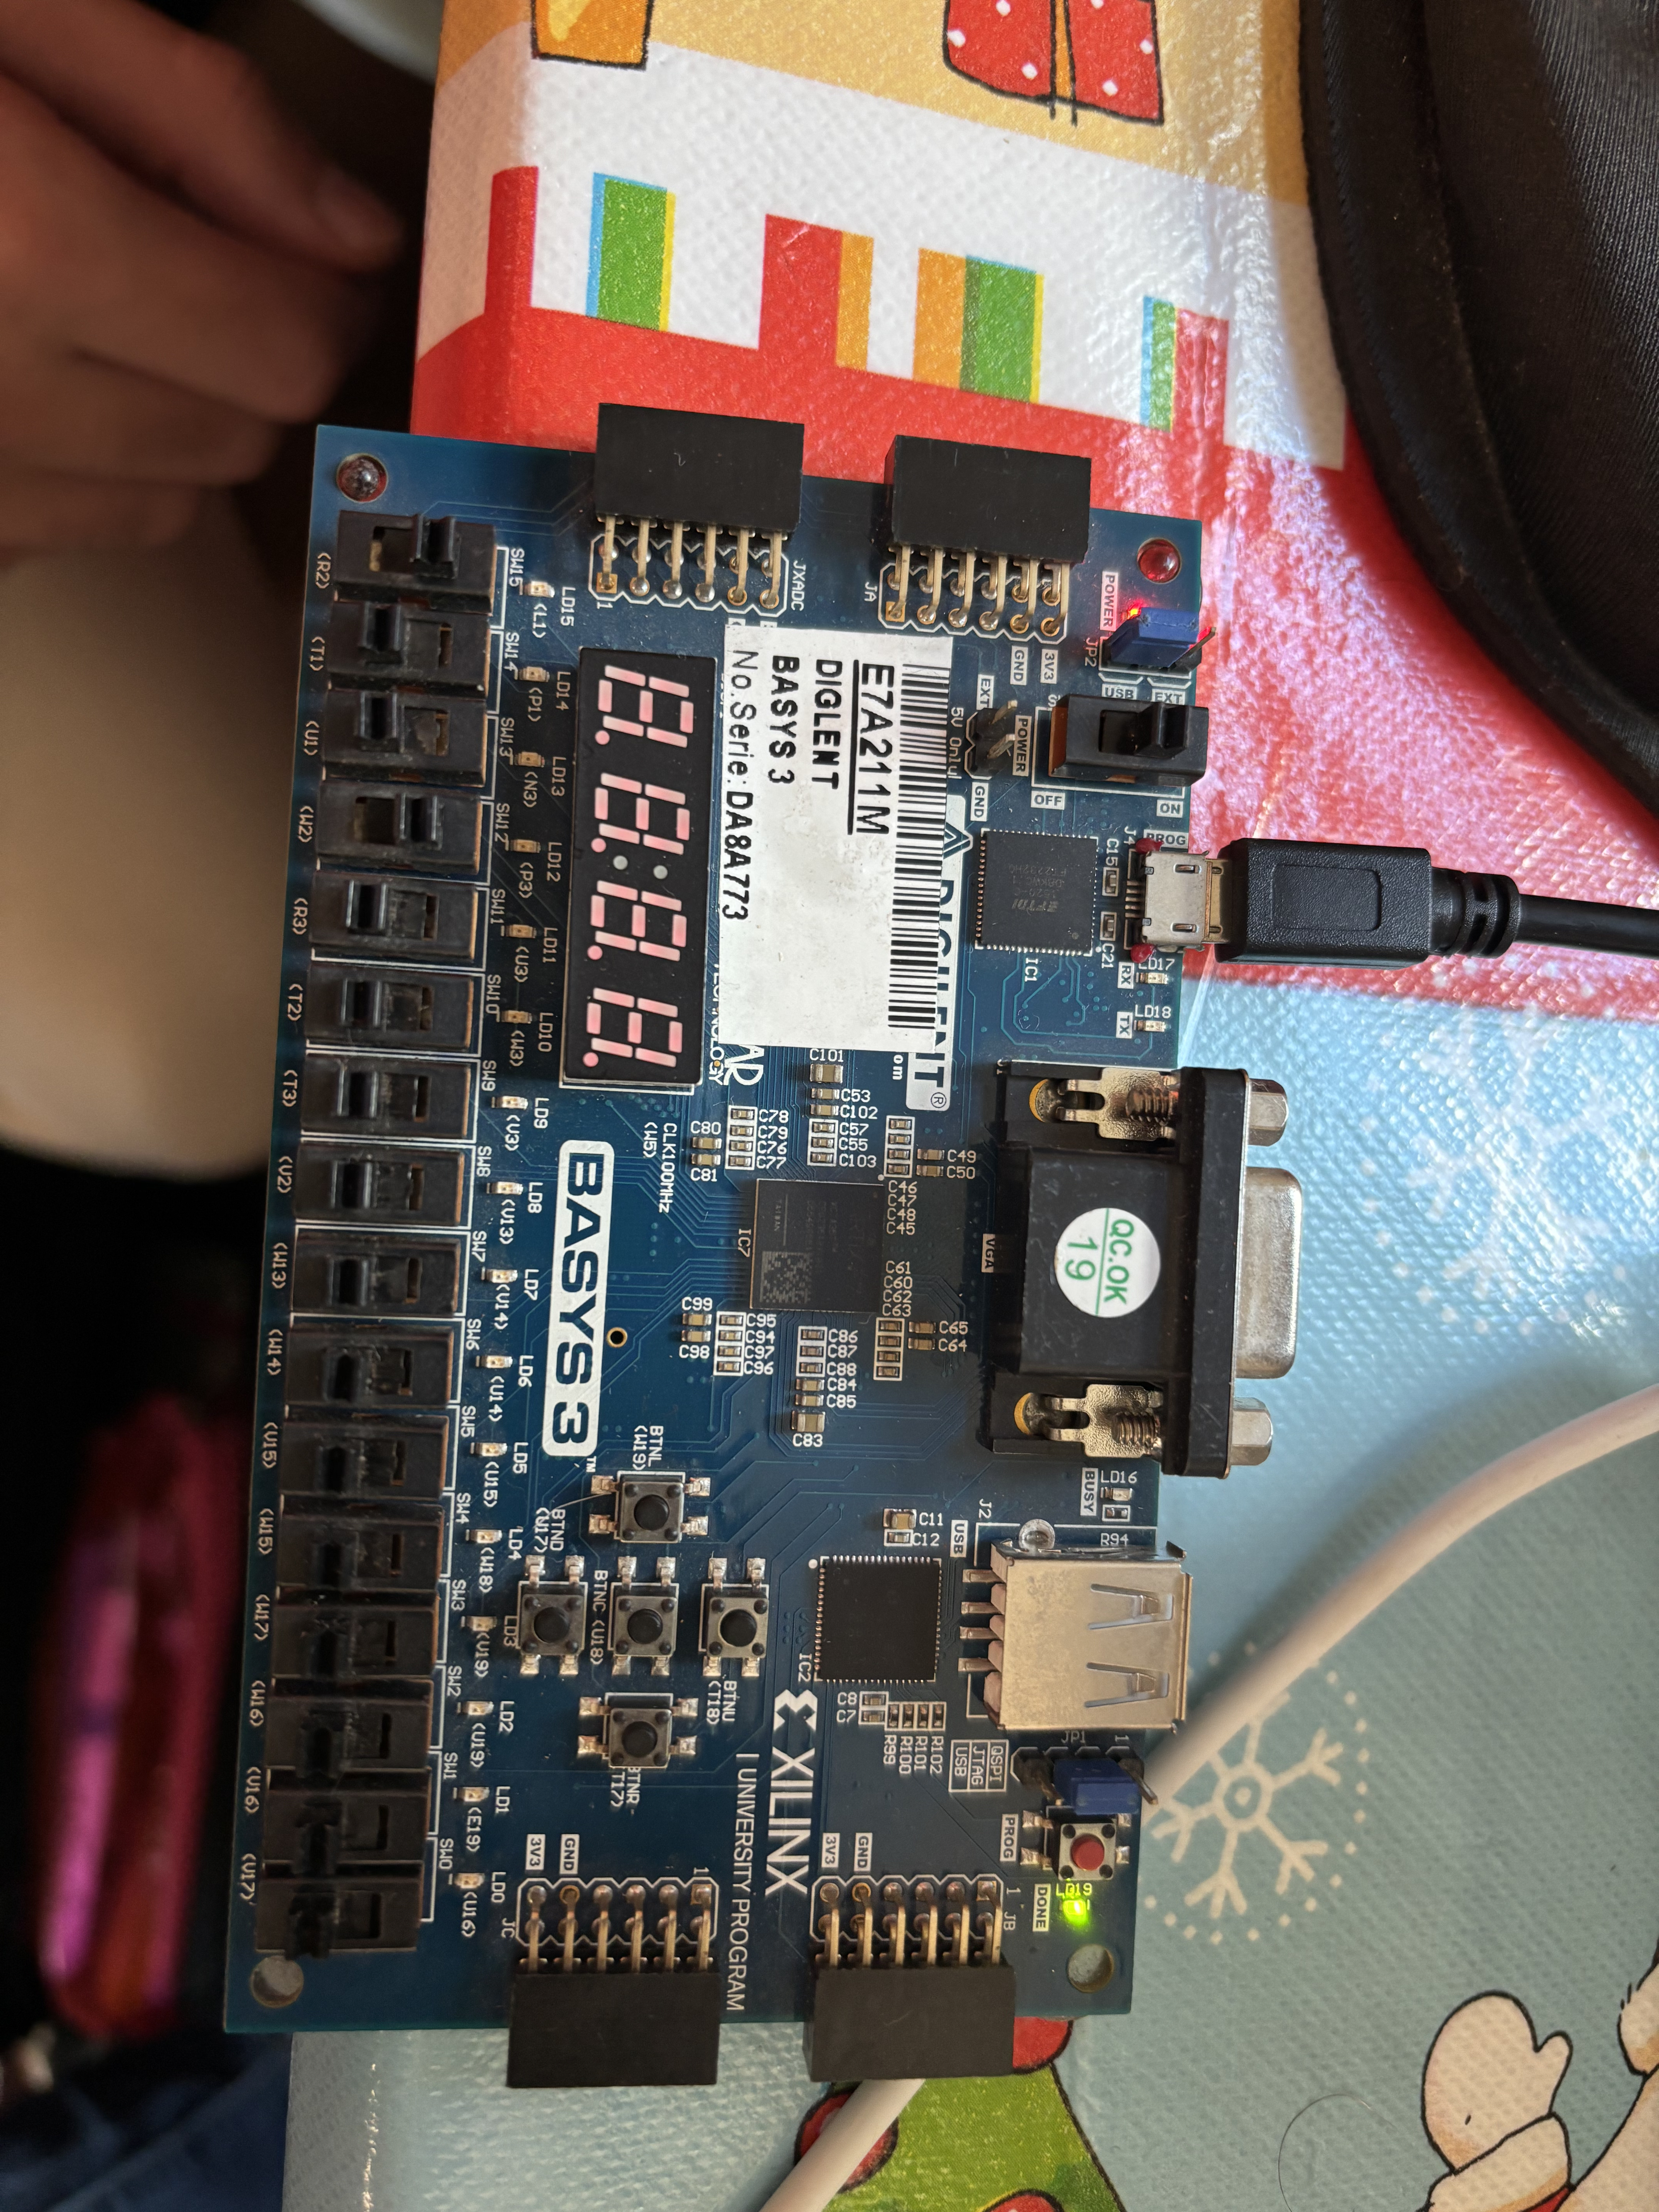
\includegraphics[width = 0.3\textwidth]{OFFCIS.jpg}
  \caption{Basys 3 Board Implementation of the Water Pump Controller when the cistern is full }
  \label{fig:CISOFF}
\end{figure}

\subsection{Coin detector}\label{Monedas}
For the coin game circuit, a combinational system was designed with three inputs (A, B, C) and a three-bit output vector (MON). This module encodes the result of a coin-based game according to the combination of selected inputs. For this circuit, the following truth table was developed, showing the relationship between the inputs and the output vector MON: 

\begin{table}[H]
\centering
\begin{tabular}{|c|c|c|c|c|}
\hline
\multicolumn{3}{|c|}{\textbf{Inputs}} & \multicolumn{2}{c|}{\textbf{Outputs}} \\
\hline
\textbf{A} & \textbf{B} & \textbf{C} & \textbf{result (ABC)} & \textbf{MON} \\ \hline
0 & 0 & 0 & 000 & 000 \\
0 & 0 & 1 & 001 & 111 \\
0 & 1 & 0 & 010 & 111 \\
0 & 1 & 1 & 011 & 111 \\
1 & 0 & 0 & 100 & 100 \\
1 & 0 & 1 & 101 & 111 \\
1 & 1 & 0 & 110 & 010 \\
1 & 1 & 1 & 111 & 001 \\ \hline
\end{tabular}
\caption{Combinations for Coin Detector }
\label{tab:Money_truth_table}
\end{table}
And based on these truth tables, a code was generated in VHDL to simulate and implement the circuit. The code is shown below:
\lstinputlisting[language=VHDL, caption=VHDL Code for Coin detector, label=lst:vhdl_juego]{codigos/VHDL/Monedas/design.vhd}
From which, the following testbench was created to verify the functionality of the code:
\lstinputlisting[language=VHDL, caption=VHDL Testbench for Coin detector, label=lst:vhdl_tb_juego]{codigos/VHDL/Monedas/testbench.vhd}
Once the truth table was verified, the corresponding VHDL code was implemented, and simulations were carried out to check its functionality. Subsequently, the circuit behavior was verified in EpWave, observing the timing and sequence of the outputs, and finally it was implemented on the Basys 3 board, where the physical outputs could be visualized through LEDs. 

\begin{figure}[H]
  \centering
  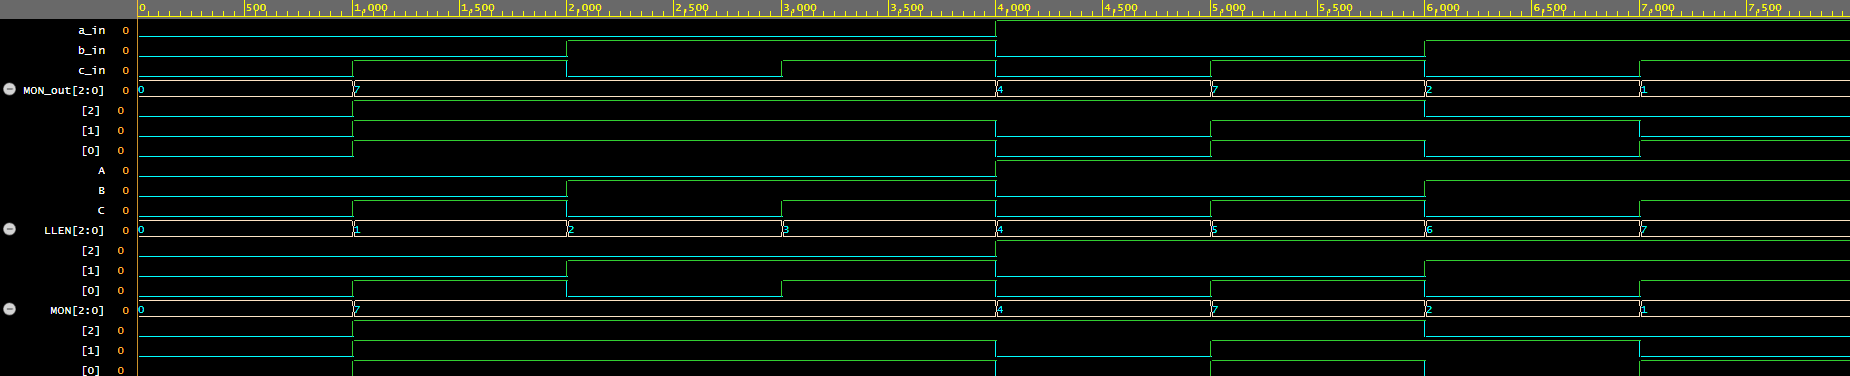
\includegraphics[width = 0.5\textwidth]{mon.png}
  \caption{EDA Waves Simulation for Coin Detector Program }
  \label{fig:lab_mon_eda}
\end{figure}
\begin{figure}[H]
  \centering
  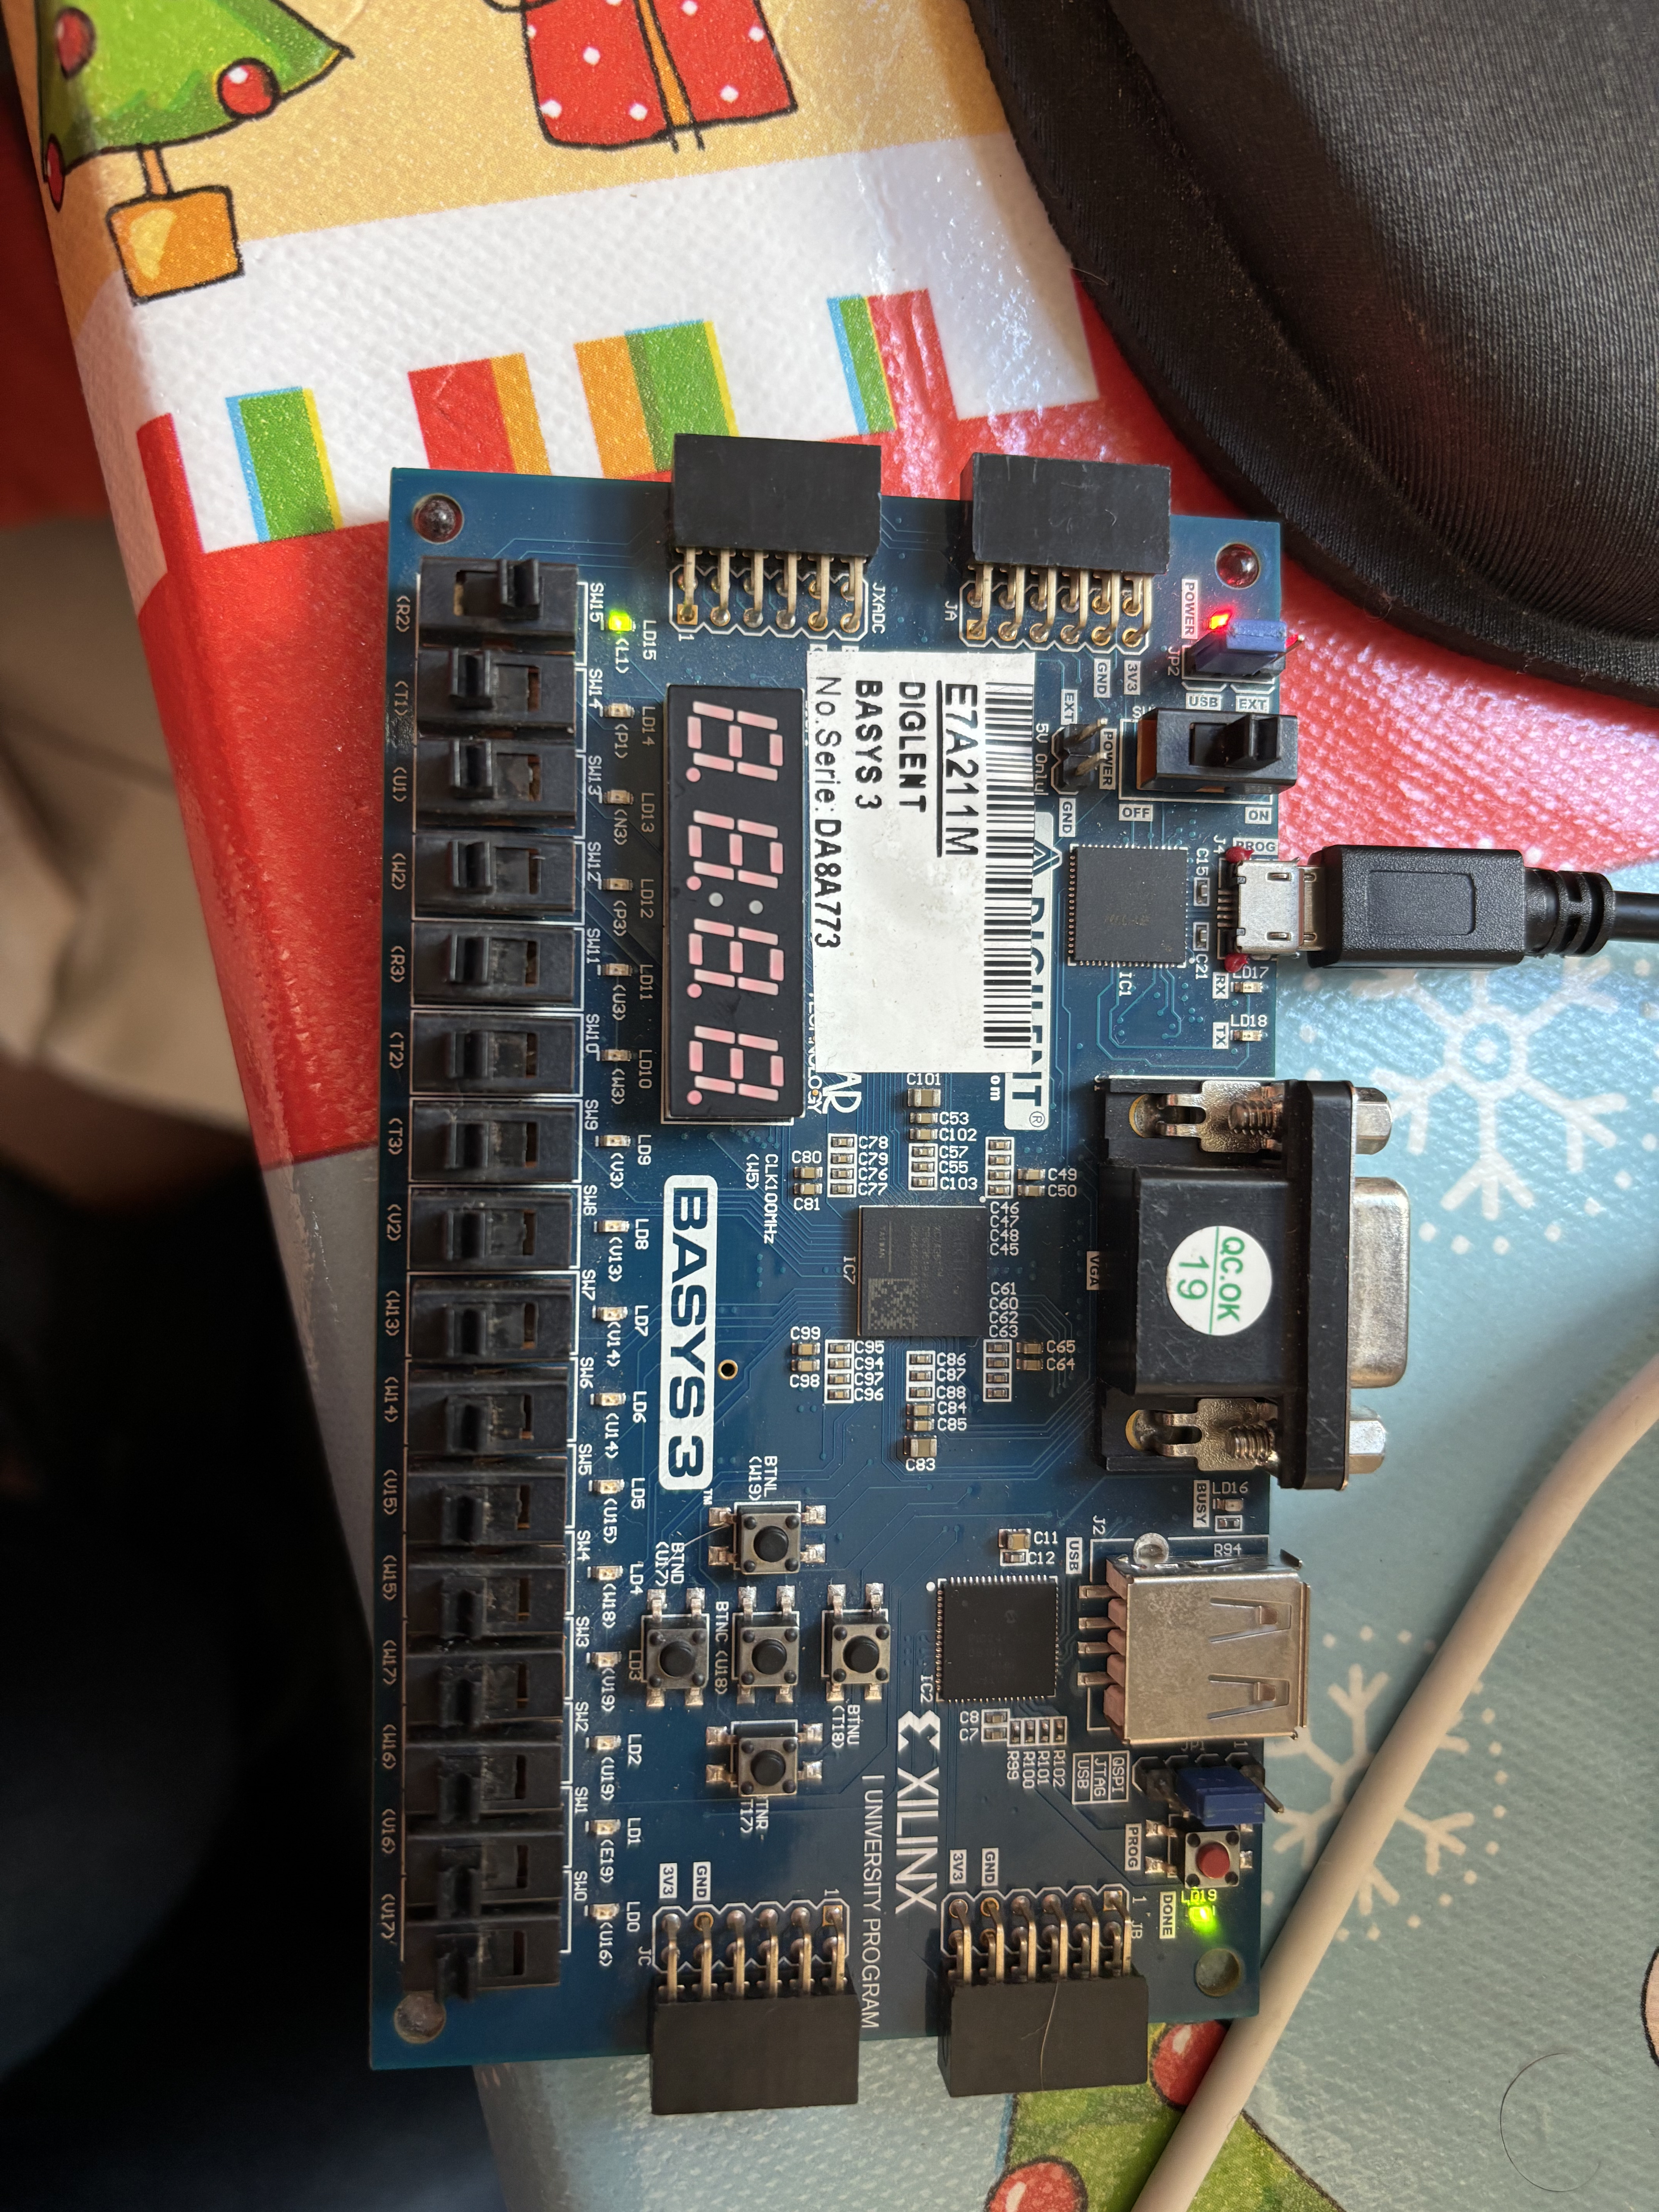
\includegraphics[width = 0.3\textwidth]{1coin.jpg}
  \caption{Basys 3 Board Implementation of the Coin Detector when \$1 is detected }
  \label{fig:1_coin}
\end{figure}
\begin{figure}[H]
  \centering
  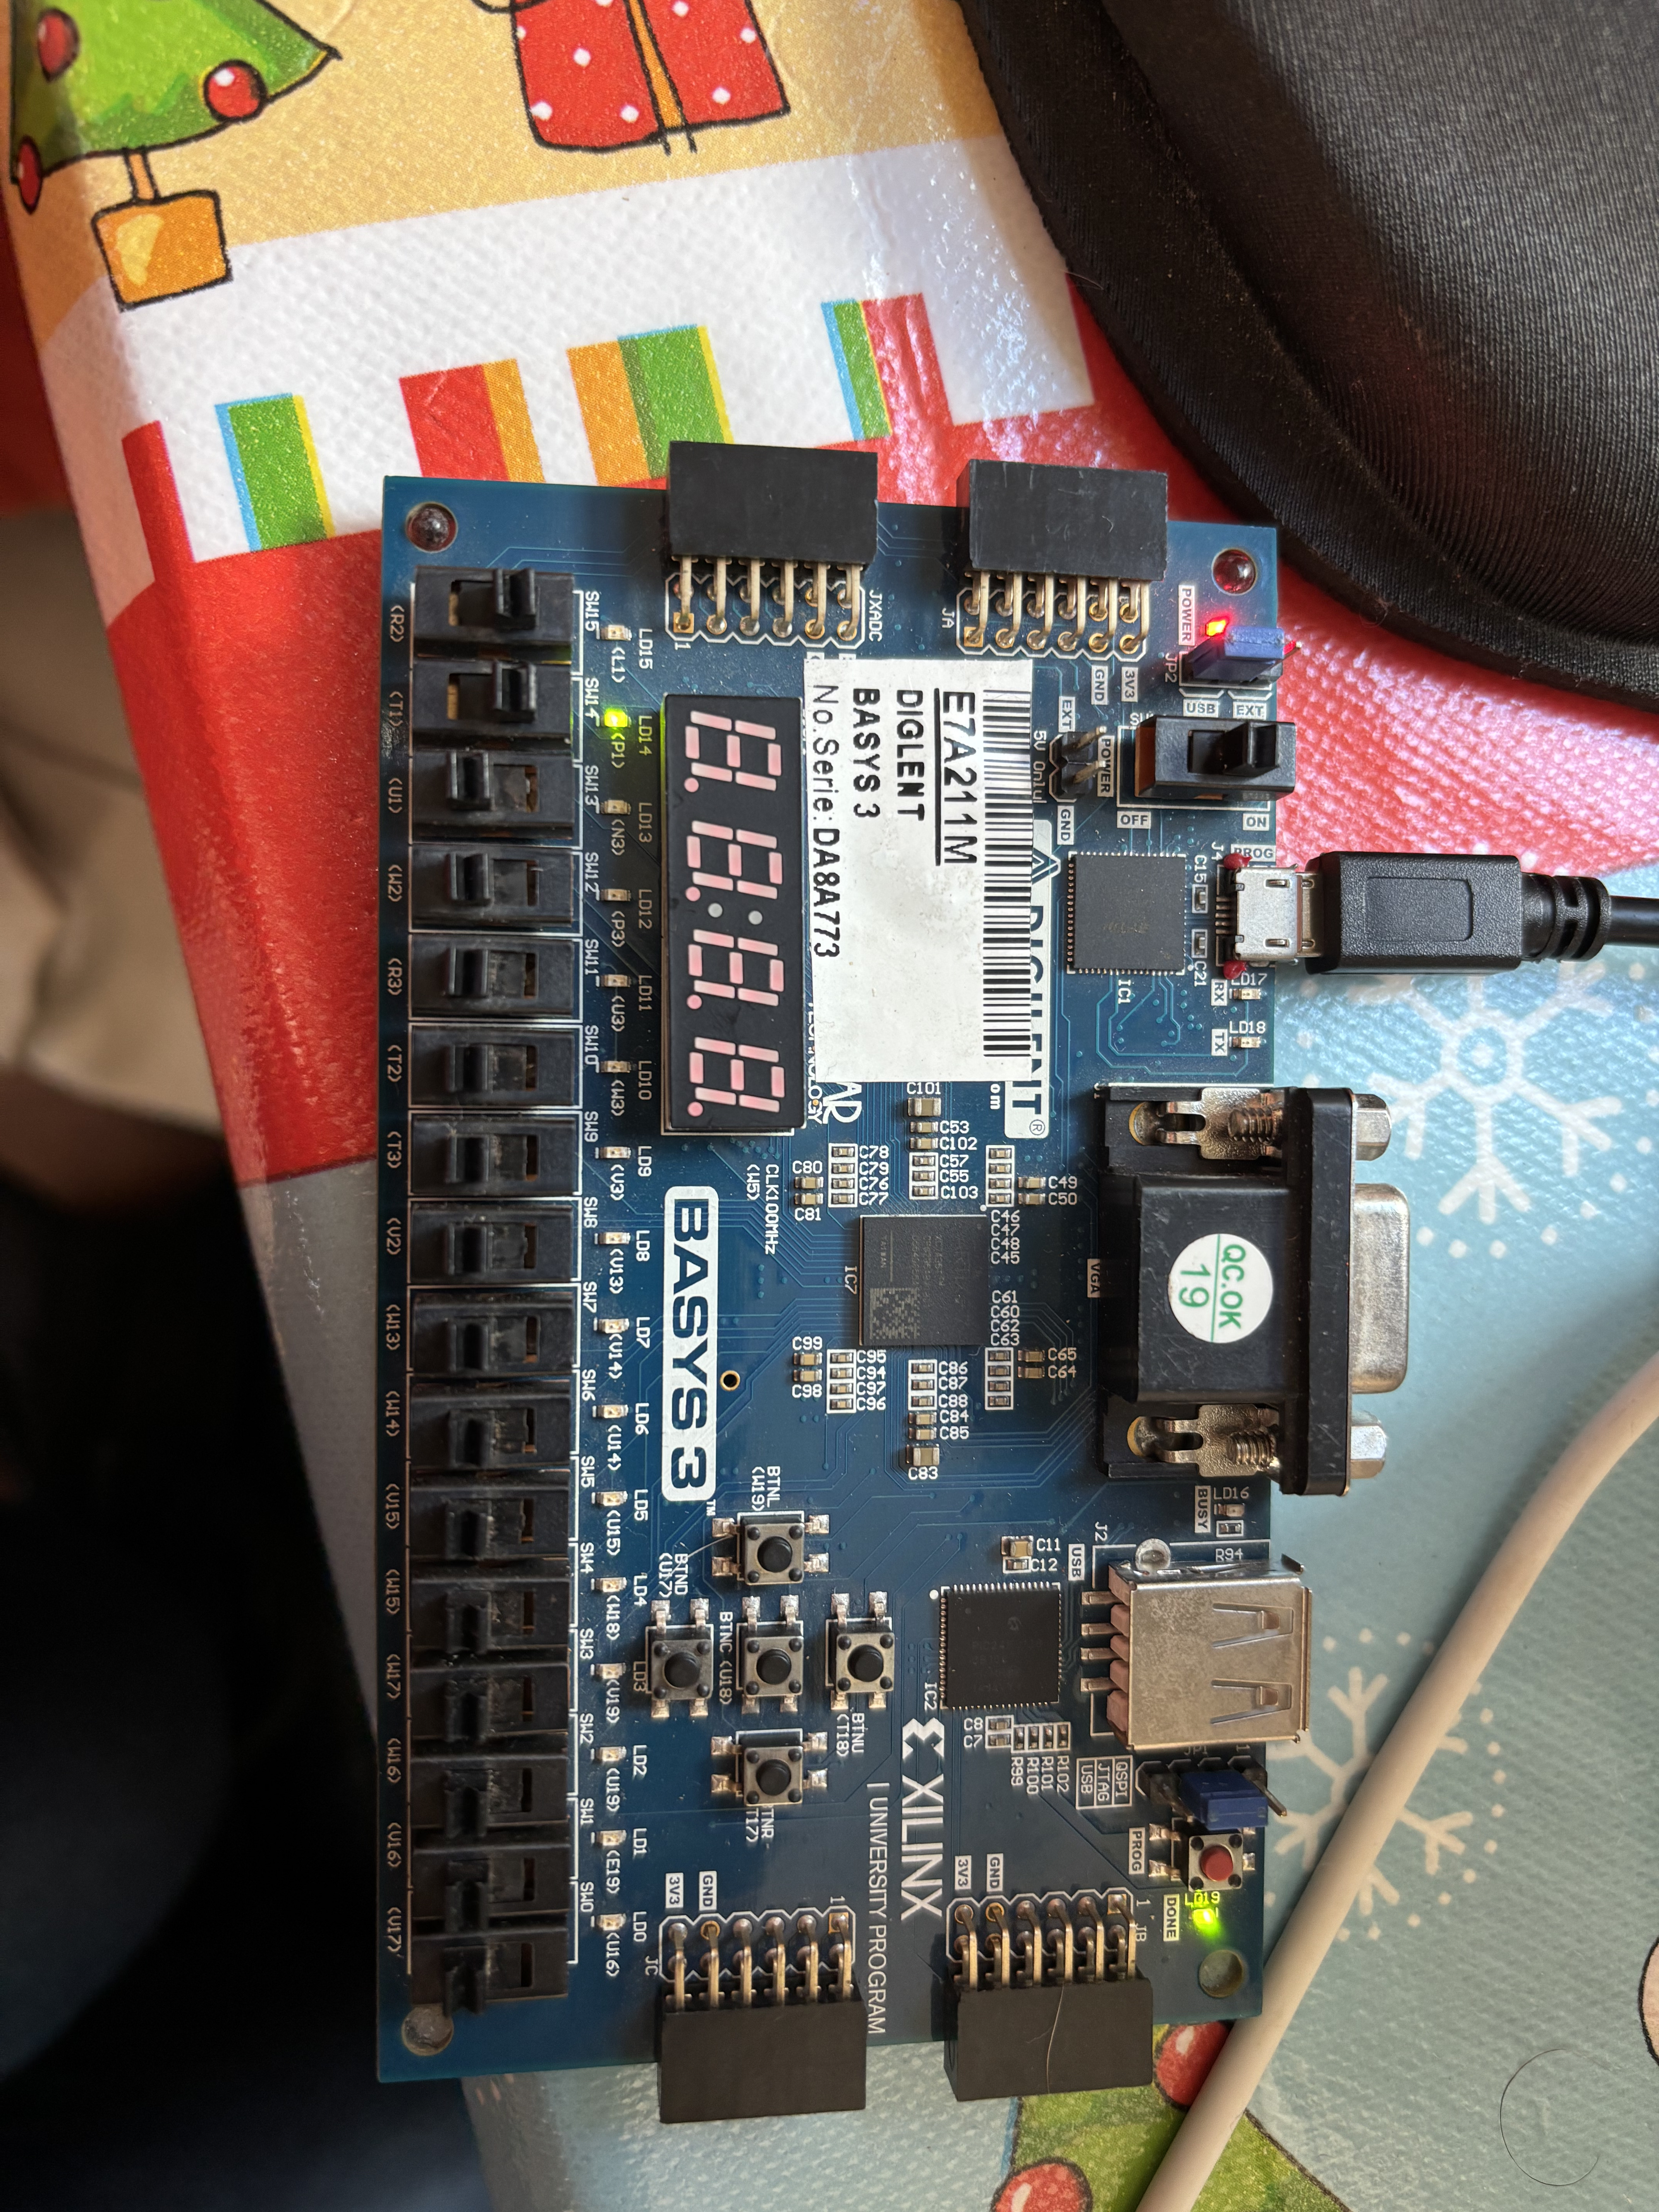
\includegraphics[width = 0.3\textwidth]{5coin.jpg}
  \caption{Basys 3 Board Implementation of the Coin Detector when \$5 is detected }
  \label{fig:5_coin}
\end{figure}
\begin{figure}[H]
  \centering
  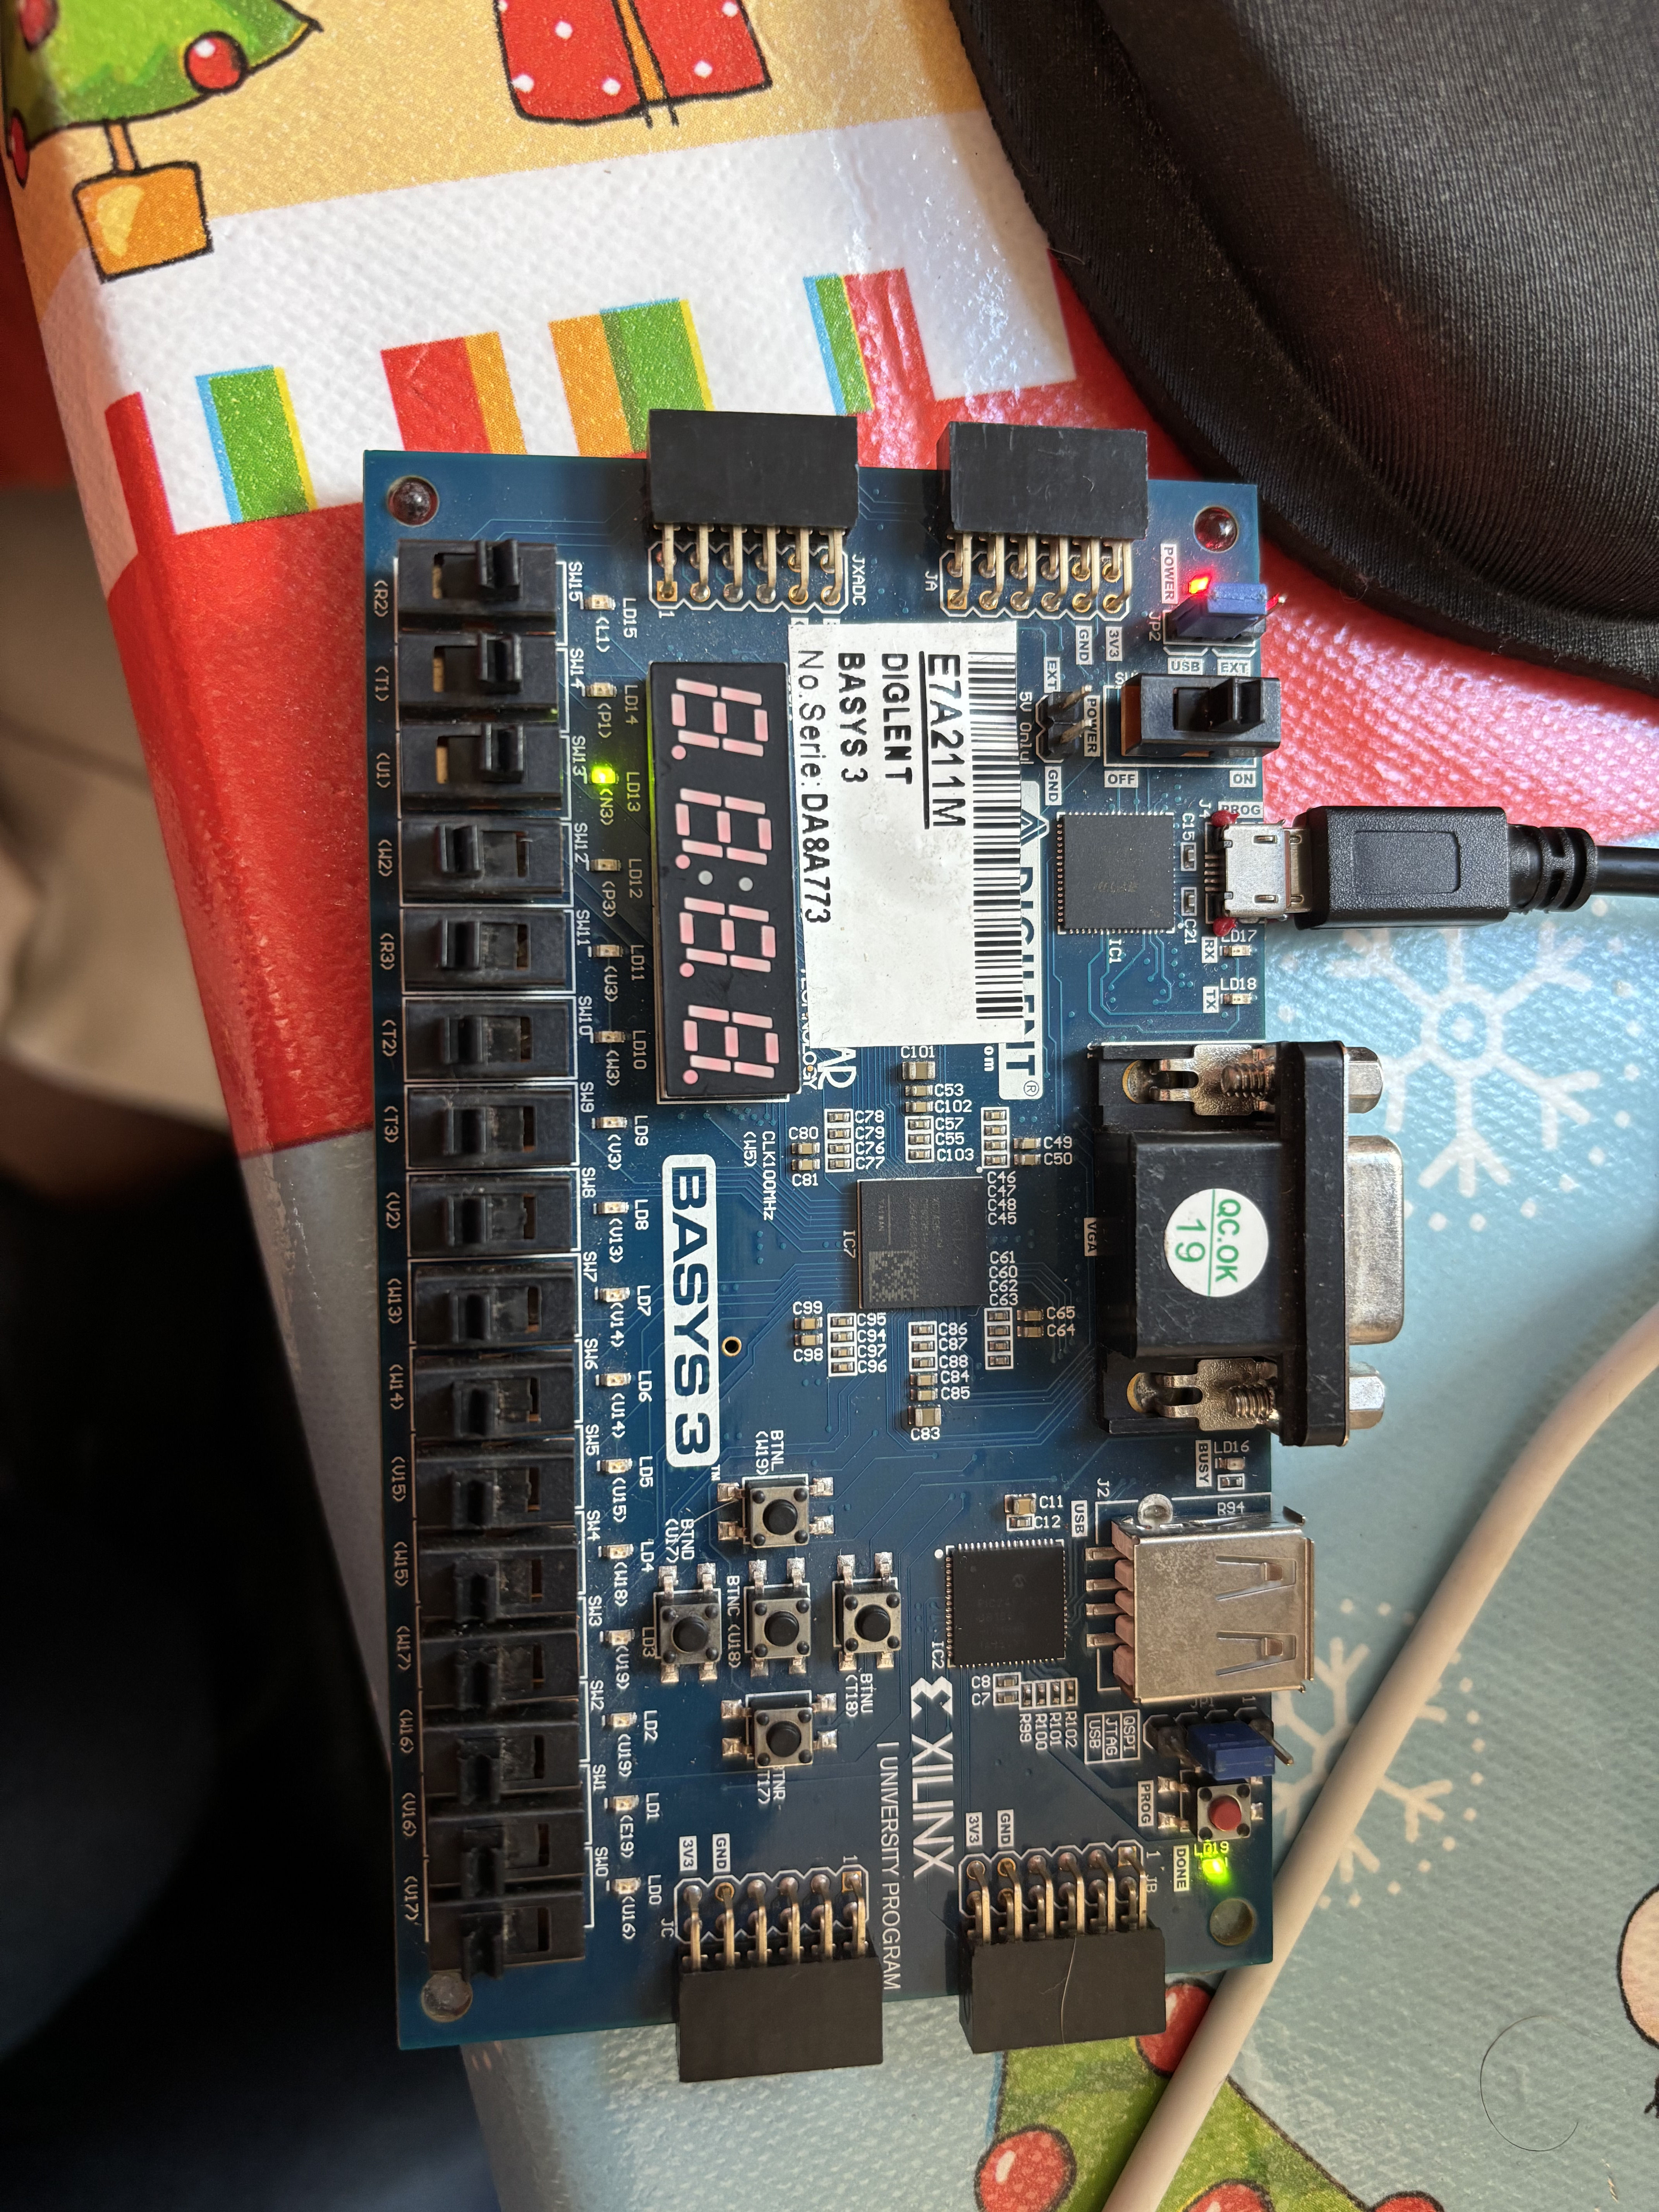
\includegraphics[width = 0.3\textwidth]{10 coin.jpg}
  \caption{Basys 3 Board Implementation of the Coin Detector when \$10 is detected }
  \label{fig:10_coin}
\end{figure}
\begin{figure}[H]
  \centering
  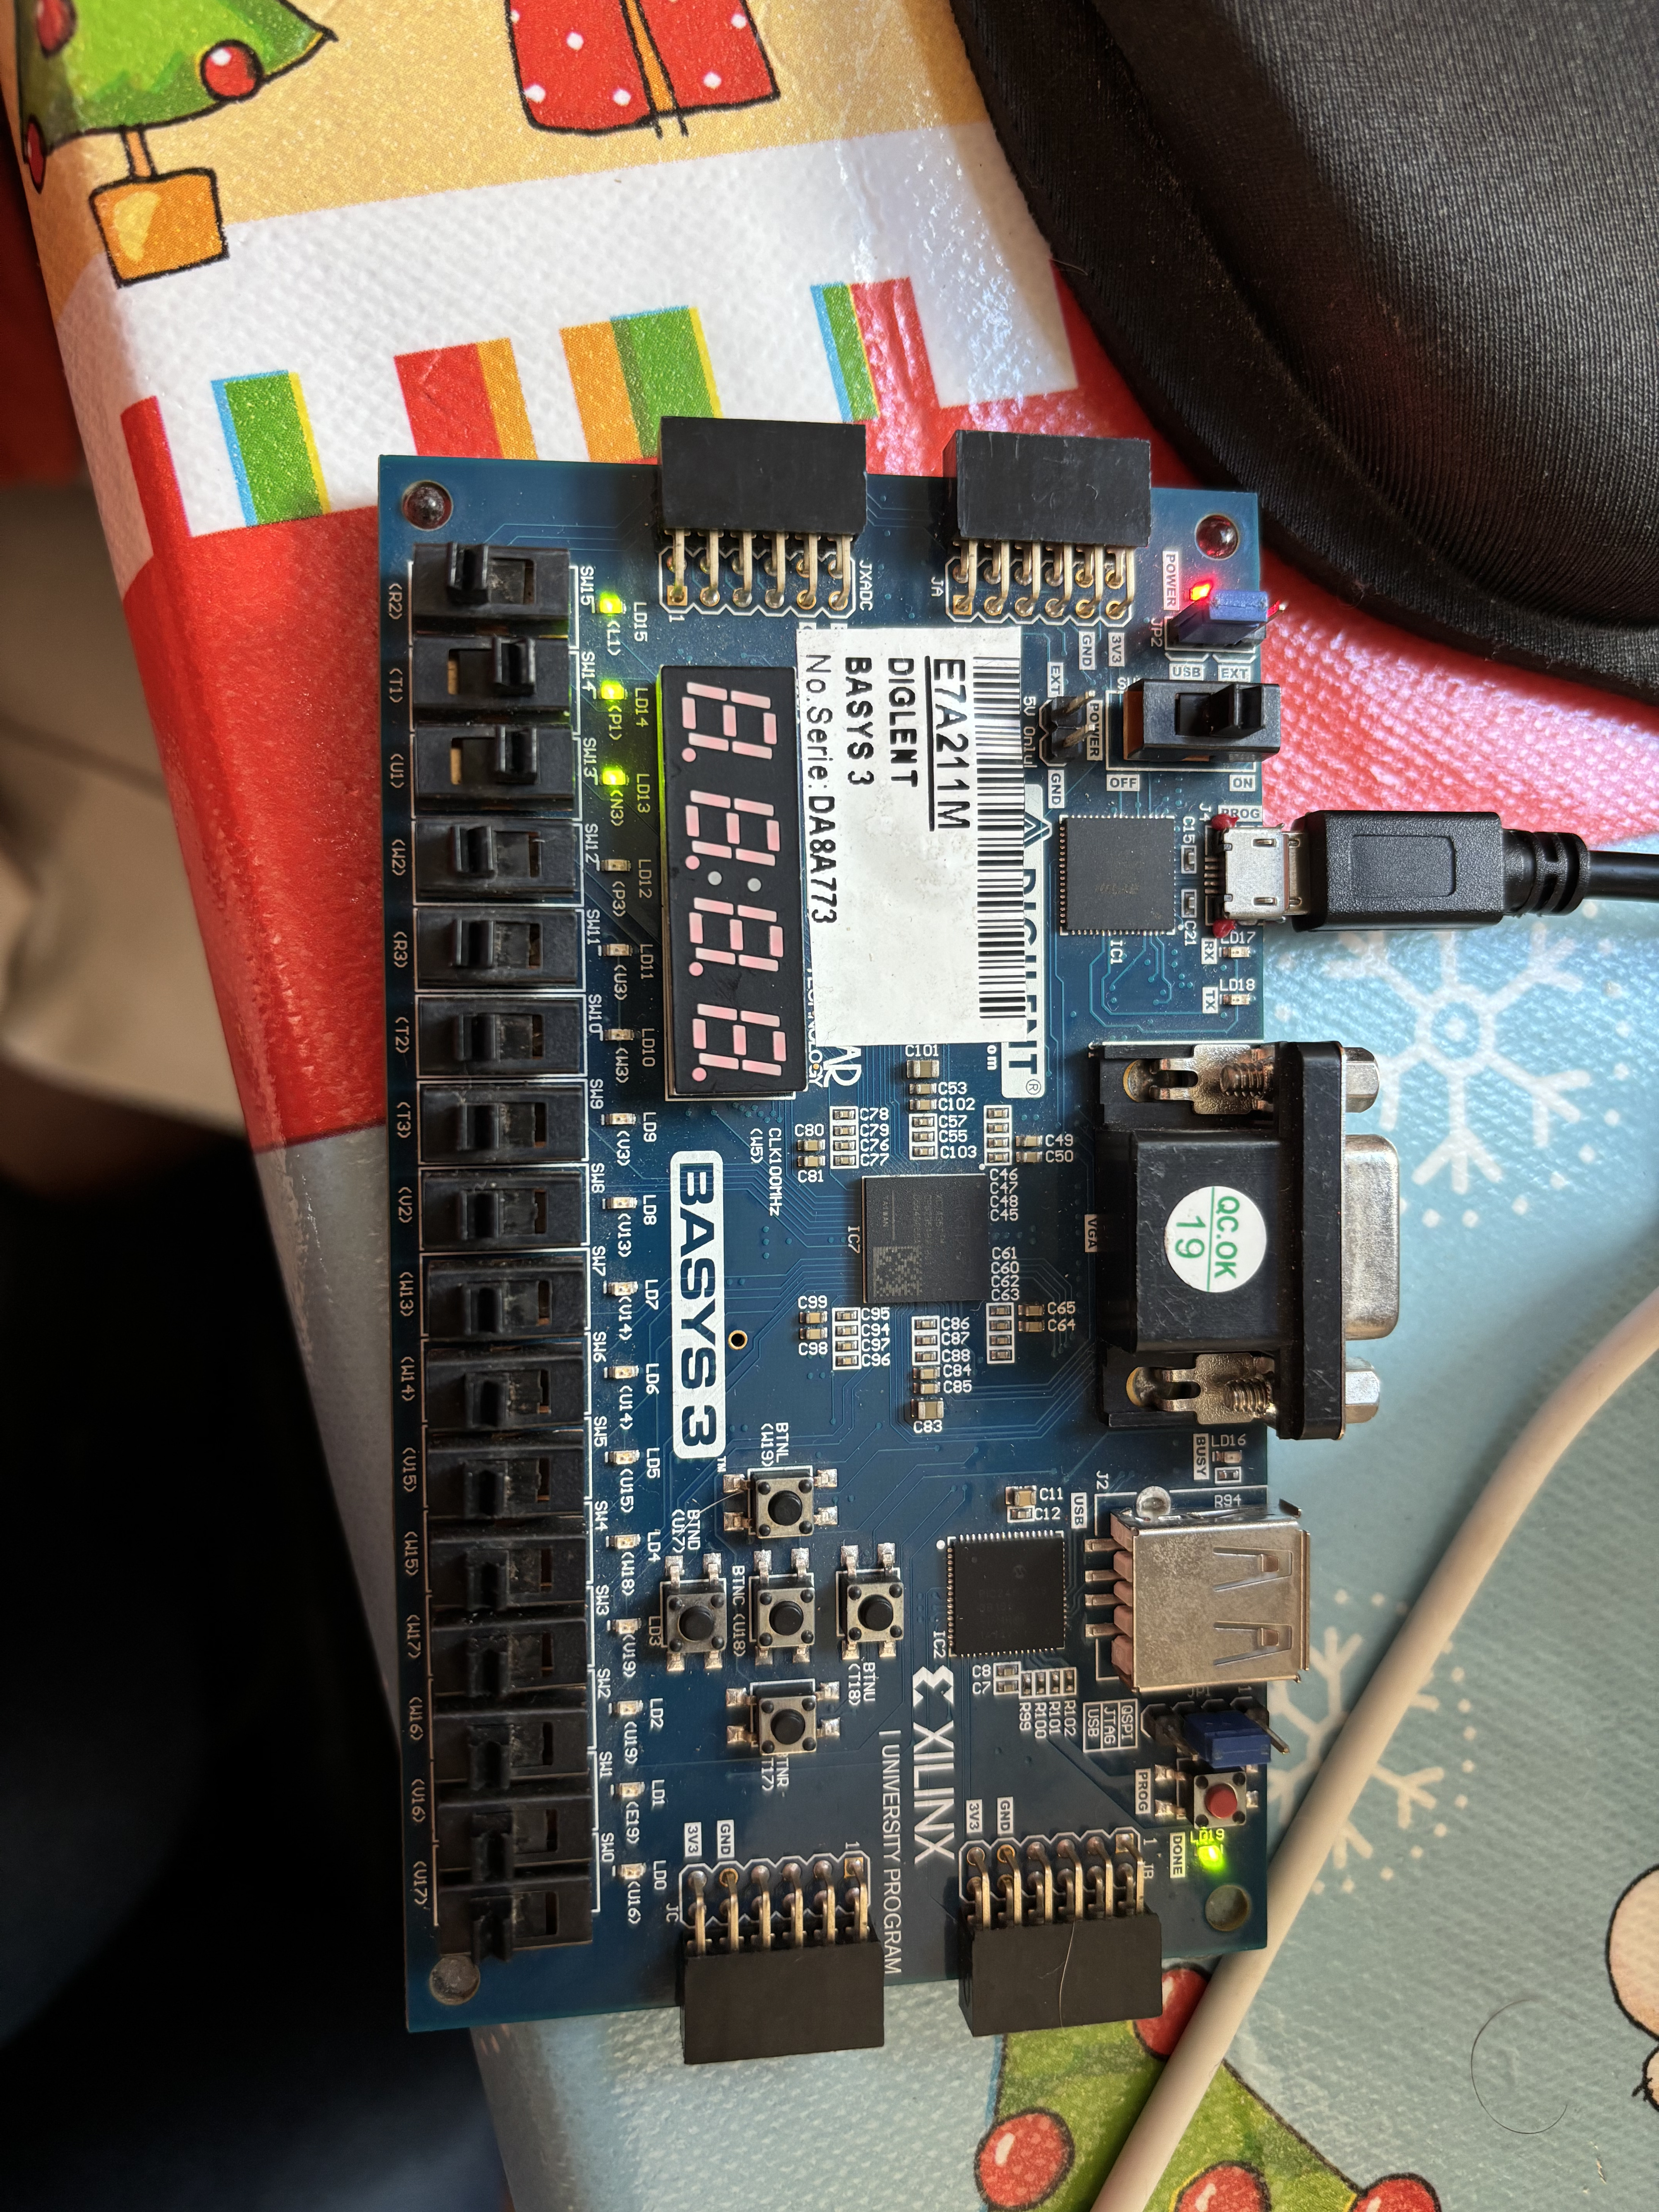
\includegraphics[width = 0.3\textwidth]{error.jpg}
  \caption{Basys 3 Board Implementation of the Coin Detector in Case of an Error }
  \label{fig:ERROR}
\end{figure}

\section{Analysis of Results}\label{Analysis}
In this laboratory practice, three combinational logic circuits were designed and verified: a water pump controller, a coin detector, and a Rock Paper Scissors game. The analysis followed the three main phases outlined in the methodology: logical analysis based on functional requirements and truth tables, VHDL simulation using EDA Playground, and physical verification on the Basys 3 board. The observed behavior in each phase is described below. 

\subsection{Rock Paper Scissors Game}
\subsubsection{Logical Analysis}
The logic for the game was defined by five inputs: a “play” button (PB) and two-bit inputs for Player A (JAA, JAB) and Player B (JBA, JBB). The system generates three mutually exclusive outputs: GJA (Player A wins) , GJB (Player B wins) , and E (tie) . As detailed in the truth tables, outputs are only processed when PB = 1. The logic correctly maps the game’s rules: GJA = 1 when Player A’s combination beats Player B’s , GJB = 1 when Player B wins , and E = 1 when both players have identical inputs . When PB = 0, all outputs remain 0. 

\subsubsection{EDA Playground Analysis}
Simulation waveforms were obtained using a testbench that systematically cycled through all possible input combinations. The output vector responded exactly as predicted: When both players’ inputs were identical and PB was active, the tie bit (E) was set. When Player A’s input represented a winning move against Player B, GJA was activated. Transitions were clean, validating the VHDL implementation. 

\subsubsection{Basys 3 Implementation}
On the Basys 3 board, switches represented player inputs and the PB button. Three LEDs were assigned to GJA, GJB, and E. Physical testing confirmed the simulation results: Player A’s winning combination illuminated GJA. Player B’s win illuminated GJB. During a tie, E was active. The immediate response of the LEDs matched the theoretical design perfectly. 

\subsection{Water Pump}
\subsubsection{Logical Analysis}
The water pump system is controlled by four sensors: A (tank high level) , B (tank low level) , C (cistern high level) , and D (cistern low level) . The single output M activates the pump motor. The primary requirement is to activate the motor (M = 1) only when the cistern is not empty AND the tank is not full. The “cistern not empty” condition is met when D = 1 (detecting water at the low level). The “tank not full” condition is met when A = 0. This leads to the simplified Boolean expression: $\mathbf{M} = \neg A \cdot D$ . The states of B and C are “don’t care” conditions for the motor activation. 

\subsubsection{EDA Playground Analysis}
Simulation in EDA Playground (Figure \ref{fig:lab_cis_eda}) used a testbench that iterated through all 16 possible sensor states. The resulting waveforms confirmed that M was high only when A = 0 and D = 1. For all other 14 combinations, the motor output remained low, precisely validating the VHDL implementation. 

\subsubsection{Basys 3 Implementation}
On the Basys 3 board, four switches represented sensors A, B, C, and D, while a single LED represented the motor M. Physical tests corroborated the logical analysis: the LED was illuminated only under the valid “ON” conditions ($\neg A \cdot D$) and remained off under all other conditions. The response of the LED to the switch positions was immediate and fully matched the simulation and derived Boolean function. 

\subsection{Coin detector}
\subsubsection{Logical Analysis}
The coin detector identifies three valid coin types using three inputs: A, B, and C. The output MON[2:0] indicates the coin type or an error state: 
Input "001" $\to$ \$1 coin $\to$ MON = 100 
Input "011" $\to$ \$5 coin $\to$ MON = 010 
Input "111" $\to$ \$10 coin $\to$ MON = 001 
Input "000" $\to$ no coin $\to$ MON = 000 
Any other combination $\to$ invalid state $\to$ MON = 111 
This logic ensures that only physically possible combinations of sensors are recognized as valid coins. 

\subsubsection{EDA Playground Analysis}
The simulation cycled through all 8 possible input combinations. Each valid combination produced the correct output, while invalid combinations triggered the error state, validating the robustness of the VHDL design against unexpected inputs. 

\subsubsection{Basys 3 Implementation}
Three switches were used for inputs A, B, and C, and three LEDs displayed the output MON. The physical tests perfectly mirrored the simulation: 
"001" activated the first LED (\$1) 
"011" activated the second LED (\$5) 
"111" activated the third LED (\$10) 
Invalid inputs activated all three LEDs simultaneously, indicating an error 
This agreement between physical testing and simulation confirmed the correct synthesis of the system. 

\section{Conclusions}\label{Conclusion}
In this laboratory practice, three combinational systems were designed, simulated, and implemented: the water pump controller, the coin detector, and the Rock-Paper-Scissors game. The experience allowed for synthesizing the knowledge gained in combinational logic, VHDL, and hardware testing. Achievements include the correct activation of the motor only under safe conditions, accurate identification of valid coins, and correct determination of the winner or a tie in the game. Minor errors were detected during testing, such as invalid input combinations, which helped reinforce the robustness of the design and adjust the output conditions. Possible improvements include optimizing the VHDL code to reduce complexity, adding protection against unexpected inputs, and extending physical tests with additional scenarios to further validate the systems. Overall, the practice strengthened skills in the design, simulation, and verification of digital systems in an integrated manner. 

% Bibliografía 
%---------------------------------------------------------------------------------------------------------------------------------------------------------------
\begin{thebibliography}{9}

\bibitem{lameres2017}
LaMeres, B. J. (2017). \textit{Introduction to Logic Circuits \& Logic Design with VHDL} (2nd ed.). Springer. (SpringerLink) 

\bibitem{vhdlwhiz}
VHDLWhiz. (n.d.). \textit{Combinational logic}. Recuperado de https://vhdlwhiz.com/terminology/combinational-logic/ (vhdlwhiz.com) 

\end{thebibliography}
% ----------------------------------------------------------------------------------------------------------------------------------------------------------------
\end{multicols}
\end{document}            
% Fin del documento